% Copyright 2010 by Frank Wood

\documentclass{beamer}
\usepackage{algorithm}
\usepackage{algorithmic}
\usepackage[numbers]{natbib}

% Setup appearance:

\usetheme{Darmstadt}
%\usetheme{Copenhagen}
\usefonttheme[onlylarge]{structurebold}
\setbeamerfont*{frametitle}{size=\normalsize,series=\bfseries}
\setbeamertemplate{navigation symbols}{}

% Standard packages

\usepackage[english]{babel}
%\usepackage[latin1]{inputenc}
%\usepackage{times}
%\usepackage[T1]{fontenc}
%\usepackage{nnfootnote}
\usepackage{amsfonts}
\usepackage{amsmath}
%\newcommand{\argmax}{\operatornamewithlimits{argmax}}
\def\newblock{\hskip .11em plus .33em minus .07em}
% Setup TikZ

%\usepackage{tikz}
%\usetikzlibrary{arrows}
%\tikzstyle{block}=[draw opacity=0.7,line width=1.4cm]


% Author, Title, etc.

\title[Fully Unsupervised Modeling of Discrete Observations of Natural Data] 
{
  A Step Towards Fully Unsupervised, Life-Long, Incremental Learning
}

\author[Wood]
{
  Frank~Wood%\inst{1}
}

\institute[Columbia University]
{
  %\inst{1}%
  Columbia University
}

\date[Google 2010]
{Google 2010}

%\def\blfootnote{\xdef\@thefnmark{}\@footnotetext}


% The main document
% !TEX root = talk.tex

\newcommand{\comment}[1]{}
%\newcommand{\comment}[1]{{\marginpar{\tiny {#1} }}}
\def\todo#1{TODO(#1)}

\def\bigO{{\mathcal O}}
\def\balpha{\mbox{\boldmath $\alpha$}}
\def\bbeta{\mbox{\boldmath $\beta$}}
\def\beeta{\mbox{\boldmath $\eta$}}
\def\blambda{\mbox{\boldmath $\lambda$}}
\def\bmu{\mbox{\boldmath $\mu$}}
\def\bphi{\mbox{\boldmath $\phi$}}
\def\bpsi{\mbox{\boldmath $\psi$}}
\def\bsigma{\mbox{\boldmath $\sigma$}}
\def\btau{\mbox{\boldmath $\tau$}}
\def\btheta{\mbox{\boldmath $\theta$}}
\def\dbphi{\dot{\mbox{\boldmath $\phi$}}}
\def\dbtau{\dot{\mbox{\boldmath $\tau$}}}
\def\dbtheta{\dot{\mbox{\boldmath $\theta$}}}

%\newcommand{\nofootnotemark}{\let\@makefnmark\relax}
\newcommand{\bX}{\mathbf{X}}
\newcommand{\bY}{\mathbf{Y}}
\newcommand{\bW}{\mathbf{W}}
\newcommand{\bZ}{\mathbf{Z}}
\newcommand{\bH}{\mathbf{H}}
\newcommand{\bQ}{\mathbf{Q}}
\newcommand{\bA}{\mathbf{A}}
\newcommand{\bI}{\mathbf{I}}
\newcommand{\by}{\mathbf{y}}
\newcommand{\bz}{\mathbf{z}}
\newcommand{\bx}{\mathbf{x}}

\newcommand{\ith}{i^\mathrm{th}}
\def\A{{\bf A}}
\def\B{{\bf B}}
\def\C{{\bf C}}
\def\D{{\bf D}}
\def\F{{\bf F}}
\def\L{{\bf L}}
\def\M{{\bf M}}
\def\W{{\bf W}}
\def\I{{\bf I}}
\def\J{{\bf J}}
\def\R{{\bf R}}
\def\U{{\bf U}}
\def\V{{\bf V}}
\def\b{{\bf b}}
\def\c{{\bf c}}
\def\d{{\bf d}}
\def\r{{\bf r}}
\def\s{{\bf s}}
\def\t{{\bf t}}
\def\u{{\bf u}}
\def\v{{\bf v}}
\def\f{{\bf f}}
\def\x{{\bf x}}
\def\y{{\bf y}}
\def\w{{\bf w}}
\def\vo{{\bf o}}
\def\p{{\bf p}}
\def\O{{\bf 0}}
%\def\a{{\bf a}}


\def\vbpsi{\vec{\mbox{\boldmath $\psi$}}} 
\def\vpsi{\vec{\psi}} 
\def\vbphi{\vec{\mbox{\boldmath $\phi$}}} 
\def\vphi{\vec{\phi}} 
\def\vbtau{\vec{\mbox{\boldmath $\tau$}}} 
\def\vbtheta{\vec{\mbox{\boldmath $\theta$}}} 
\def\vD{\vec{D}}
\def\vf{\vec{\bf f}}
\def\vF{\vec{\bf F}}
\def\vI{\vec{\bf I}}
\def\vR{\vec{\bf R}}
\def\vv{\vec{v}}
\def\vV{\vec{\bf V}}

\def\pon{p_{\mathrm{on}}}
\def\poff{p_{\mathrm{off}}}

\def\tr{^{\text{T}}}

%%% Vector notation for sections 3 and 4
%%% Vector notation for sections 3 and 4
\def\mvec{\vec{m}}
\def\fvec{\vec{f}}
\def\appfvec{\vec{f}_k}
\def\avec{\vec{a}}
\def\bvec{\vec{b}}
\def\evec{\vec{e}}
\def\uvec{\vec{u}}
\def\xvec{\vec{x}}
\def\wvec{\vec{w}}
\def\gradvec{\vec{\nabla}}

\def\aM{\mbox{\bf a}_M}
\def\aS{\mbox{\bf a}_S}
\def\aO{\mbox{\bf a}_O}
\def\aL{\mbox{\bf a}_L}
\def\aP{\mbox{\bf a}_P}
\def\ai{\mbox{\bf a}_i}
\def\aj{\mbox{\bf a}_j}
\def\an{\mbox{\bf a}_n}
\def\a1{\mbox{\bf a}_1}
\def\a2{\mbox{\bf a}_2}
\def\a3{\mbox{\bf a}_3}
\def\a4{\mbox{\bf a}_4}

%\def\x{\mbox{\bf x\/}}
%\def\X{\mbox{\bf X}}
%\def\A{\mbox{\bf A}}
%\def\P{\mbox{\bf P}}
%\def\C{\mbox{\bf C}}
%\def\c{\mbox{\bf c}}
%\def\b{\mbox{\bf b}}
%\def\o{\mbox{\bf o}}
%\def\h{\mbox{\bf h}}
%\def\f{\mbox{\bf f}}
%\def\x{\mbox{\bf x}}
%\def\sx{\mbox{\scriptsize\bf x}}
%\def\z{\mbox{\bf z}}
%\def\l{\mbox{\bf l}}
%\def\m{\mbox{\bf m}}
%\def\bi{\mbox{\bf i}}
%\def\u{\mbox{\bf u}}
%\def\v{\mbox{\bf v}}
\def\a{\mbox{\bf a}}
%\def\p{\mbox{\bf p}}
%\def\r{\mbox{\bf r}}
%\def\d{\mbox{\bf d}}
%\def\Q{\mbox{\bf Q}}
%\def\s{\mbox{\bf s}}
%\def\st{\mbox{\scriptsize\bf t}}
%\def\ss{\mbox{\scriptsize\bf s}}
%\def\t{\mbox{\bf t}}
%\def\cR{{\cal R}}
%\def\calD{{\cal D}}
%\def\calS{{\cal S}}
%\def\g{\mbox{\bf g}}
%\def\e{\mbox{\bf e}}
%\def\flow{\{\mbox{\bf u}\}}
%\def\appearChange{iconic change}

\def\sigmae{\sigma}
\def\sigmam{\sigma}

\newcommand{\eg}{e.\thinspace{}g.,\@\xspace}
\newcommand{\egn}{e.\thinspace{}g.\@\xspace}
\newcommand{\cf}{cf.\@\xspace}
\newcommand{\ie}{i.\thinspace{}e.,\@\xspace}
\newcommand{\ien}{i.\thinspace{}e.\@\xspace}
\newcommand{\iid}{i.\thinspace{}i.\thinspace{}d.\@\xspace}


%\newcommand{\comment}[1]{}
\newcommand{\ponedec}{\mathcal{P}^\downarrow_1}
\newcommand{\pone}{\mathcal{P}_1}
\newcommand{\rank}[1]{\mathrm{RANK}\left[#1\right]}
\newcommand{\E}[1]{\mathrm{E}\left[#1\right]}
%\newcommand{\PY}{\mathcal{PY}}
%\newcommand{\DP}{\mathcal{DP}}
%\newcommand{\iid}{iid.}
\newcommand{\drawiid}{\stackrel{\text{iid}}{\sim}}
\newcommand{\vect}[1]{\mathbf{#1}}
\newcommand{\indicator}[1]{\text{I}\left[ #1 \right]}
\newcommand{\pdcoag}{PD(d_1,0)-\text{COAG}}
%\newcommand{\todo}{\textbf{*TODO*}}
\newcommand{\igram}{\text{$\infty$-gram}}
\newcommand{\Prob}{\text{P}}

\def\mm{sequence memoizer }
\def\MM{SM }

\def\pibf{{\boldsymbol{\pi}}}
\def\kapbf{\boldsymbol{\kappa}}
\def\taubf{\boldsymbol{\tau}}
\def\thebf{\boldsymbol{\theta}}
\def\rhobf{\boldsymbol{\rho}}
\def\phibf{\boldsymbol{\phi}}
\def\pbf{\mathbf{p}}
\def\qbf{\mathbf{q}}
\def\sbf{\mathbf{s}}
\def\tbf{\mathbf{t}}
\def\ybf{\mathbf{y}}
\def\ubf{\mathbf{u}}
\def\Ave{\mathbb{E}}

\def\wbf{\mathbf{w}}
\def\xbf{\mathbf{x}}
\def\rbf{\mathbf{r}}
\def\tbf{\mathbf{t}}
\def\kbf{\mathbf{k}}
\def\Xbf{\mathbf{X}}
\def\0bf{\mathbf{0}}
\def\Ibf{\mathbf{I}}
\def\phibf{\mathbf{\phi}}
\def\Phibf{\mathbf{\Phi}}
\def\disteq{{\stackrel{D}{=}}}
\def\EE{{\mathbb{E}}}
\def\GG{\mathcal{G}}
\def\G{G}
\def\U{U}

\def\phiv{\varphi}
\def\phivbf{\boldsymbol{\varphi}}

\def\Ocal{\mathcal{O}}
\DeclareMathOperator*{\Var}{Var}

\DeclareMathOperator*{\Bet}{Beta}
\DeclareMathOperator{\coag}{COAG}
\DeclareMathOperator{\frag}{FRAG}
\DeclareMathOperator*{\rnk}{RANK}
\DeclareMathOperator*{\gem}{GEM}
\DeclareMathOperator*{\pd}{PD}
\DeclareMathOperator*{\py}{PY}
\DeclareMathOperator*{\DP}{DP}
\DeclareMathOperator*{\PY}{PY}
\DeclareMathOperator*{\gd}{GDir}
\DeclareMathOperator*{\Dir}{Dir}
\DeclareMathOperator*{\CRP}{CRP}
\DeclareMathOperator*{\argmax}{argmax}



%%% Local Variables: 
%%% mode: latex
%%% TeX-master: "paper"
%%% End: 
% !TEX root = talk.tex
%
%\newcommand{\comment}[1]{}
%%\newcommand{\comment}[1]{{\marginpar{\tiny {#1} }}}
%
%\def\bigO{{\mathcal O}}
%\def\balpha{\mbox{\boldmath $\alpha$}}
%\def\bbeta{\mbox{\boldmath $\beta$}}
%\def\beeta{\mbox{\boldmath $\eta$}}
%\def\blambda{\mbox{\boldmath $\lambda$}}
%\def\bmu{\mbox{\boldmath $\mu$}}
%\def\bphi{\mbox{\boldmath $\phi$}}
%\def\bpsi{\mbox{\boldmath $\psi$}}
%\def\bsigma{\mbox{\boldmath $\sigma$}}
%\def\btau{\mbox{\boldmath $\tau$}}
%\def\btheta{\mbox{\boldmath $\theta$}}
%\def\dbphi{\dot{\mbox{\boldmath $\phi$}}}
%\def\dbtau{\dot{\mbox{\boldmath $\tau$}}}
%\def\dbtheta{\dot{\mbox{\boldmath $\theta$}}}
%
%%\newcommand{\nofootnotemark}{\let\@makefnmark\relax}
%\newcommand{\bX}{\mathbf{X}}
%\newcommand{\bY}{\mathbf{Y}}
%\newcommand{\bW}{\mathbf{W}}
%\newcommand{\bZ}{\mathbf{Z}}
%\newcommand{\bH}{\mathbf{H}}
%\newcommand{\bQ}{\mathbf{Q}}
%\newcommand{\bA}{\mathbf{A}}
%\newcommand{\bI}{\mathbf{I}}
%\newcommand{\by}{\mathbf{y}}
%\newcommand{\bz}{\mathbf{z}}
%\newcommand{\bx}{\mathbf{x}}
%
%\newcommand{\ith}{i^\mathrm{th}}
%\def\A{{\bf A}}
%\def\B{{\bf B}}
%\def\C{{\bf C}}
%\def\D{{\bf D}}
%\def\F{{\bf F}}
%\def\L{{\bf L}}
%\def\M{{\bf M}}
%\def\W{{\bf W}}
%\def\I{{\bf I}}
%\def\J{{\bf J}}
%\def\R{{\bf R}}
%\def\U{{\bf U}}
%\def\V{{\bf V}}
%\def\b{{\bf b}}
%\def\c{{\bf c}}
%\def\d{{\bf d}}
%\def\r{{\bf r}}
%\def\s{{\bf s}}
%\def\t{{\bf t}}
%\def\u{{\bf u}}
%\def\v{{\bf v}}
%\def\f{{\bf f}}
%\def\x{{\bf x}}
%\def\y{{\bf y}}
%\def\w{{\bf w}}
%\def\vo{{\bf o}}
%\def\p{{\bf p}}
%\def\O{{\bf 0}}
%%\def\a{{\bf a}}
%
%
%\def\vbpsi{\vec{\mbox{\boldmath $\psi$}}} 
%\def\vpsi{\vec{\psi}} 
%\def\vbphi{\vec{\mbox{\boldmath $\phi$}}} 
%\def\vphi{\vec{\phi}} 
%\def\vbtau{\vec{\mbox{\boldmath $\tau$}}} 
%\def\vbtheta{\vec{\mbox{\boldmath $\theta$}}} 
%\def\vD{\vec{D}}
%\def\vf{\vec{\bf f}}
%\def\vF{\vec{\bf F}}
%\def\vI{\vec{\bf I}}
%\def\vR{\vec{\bf R}}
%\def\vv{\vec{v}}
%\def\vV{\vec{\bf V}}
%
%\def\pon{p_{\mathrm{on}}}
%\def\poff{p_{\mathrm{off}}}
%
%\def\tr{^{\text{T}}}
%
%%%% Vector notation for sections 3 and 4
%%%% Vector notation for sections 3 and 4
%\def\mvec{\vec{m}}
%\def\fvec{\vec{f}}
%\def\appfvec{\vec{f}_k}
%\def\avec{\vec{a}}
%\def\bvec{\vec{b}}
%\def\evec{\vec{e}}
%\def\uvec{\vec{u}}
%\def\xvec{\vec{x}}
%\def\wvec{\vec{w}}
%\def\gradvec{\vec{\nabla}}
%
%\def\aM{\mbox{\bf a}_M}
%\def\aS{\mbox{\bf a}_S}
%\def\aO{\mbox{\bf a}_O}
%\def\aL{\mbox{\bf a}_L}
%\def\aP{\mbox{\bf a}_P}
%\def\ai{\mbox{\bf a}_i}
%\def\aj{\mbox{\bf a}_j}
%\def\an{\mbox{\bf a}_n}
%\def\a1{\mbox{\bf a}_1}
%\def\a2{\mbox{\bf a}_2}
%\def\a3{\mbox{\bf a}_3}
%\def\a4{\mbox{\bf a}_4}
%
%%\def\x{\mbox{\bf x\/}}
%%\def\X{\mbox{\bf X}}
%%\def\A{\mbox{\bf A}}
%%\def\P{\mbox{\bf P}}
%%\def\C{\mbox{\bf C}}
%%\def\c{\mbox{\bf c}}
%%\def\b{\mbox{\bf b}}
%%\def\o{\mbox{\bf o}}
%%\def\h{\mbox{\bf h}}
%%\def\f{\mbox{\bf f}}
%%\def\x{\mbox{\bf x}}
%%\def\sx{\mbox{\scriptsize\bf x}}
%%\def\z{\mbox{\bf z}}
%%\def\l{\mbox{\bf l}}
%%\def\m{\mbox{\bf m}}
%%\def\bi{\mbox{\bf i}}
%%\def\u{\mbox{\bf u}}
%%\def\v{\mbox{\bf v}}
%\def\a{\mbox{\bf a}}
%%\def\p{\mbox{\bf p}}
%%\def\r{\mbox{\bf r}}
%%\def\d{\mbox{\bf d}}
%%\def\Q{\mbox{\bf Q}}
%%\def\s{\mbox{\bf s}}
%%\def\st{\mbox{\scriptsize\bf t}}
%%\def\ss{\mbox{\scriptsize\bf s}}
%%\def\t{\mbox{\bf t}}
%%\def\cR{{\cal R}}
%%\def\calD{{\cal D}}
%%\def\calS{{\cal S}}
%%\def\g{\mbox{\bf g}}
%%\def\e{\mbox{\bf e}}
%%\def\flow{\{\mbox{\bf u}\}}
%%\def\appearChange{iconic change}
%
%\def\sigmae{\sigma}
%\def\sigmam{\sigma}
%
%\newcommand{\eg}{e.\thinspace{}g.,\@\xspace}
%\newcommand{\egn}{e.\thinspace{}g.\@\xspace}
%\newcommand{\cf}{cf.\@\xspace}
%\newcommand{\ie}{i.\thinspace{}e.,\@\xspace}
%\newcommand{\ien}{i.\thinspace{}e.\@\xspace}
%\newcommand{\iid}{i.\thinspace{}i.\thinspace{}d.\@\xspace}
%
%
%%\newcommand{\comment}[1]{}
%\newcommand{\ponedec}{\mathcal{P}^\downarrow_1}
%\newcommand{\pone}{\mathcal{P}_1}
%\newcommand{\rank}[1]{\mathrm{RANK}\left[#1\right]}
%%\newcommand{\E}[1]{\mathrm{E}\left[#1\right]}
%%\newcommand{\PY}{\mathcal{PY}}
%%\newcommand{\DP}{\mathcal{DP}}
%%\newcommand{\iid}{iid.}
%\newcommand{\drawiid}{\stackrel{\text{iid}}{\sim}}
%\newcommand{\vect}[1]{\mathbf{#1}}
%\newcommand{\indicator}[1]{\text{I}\left[ #1 \right]}
%\newcommand{\pdcoag}{PD(d_1,0)-\text{COAG}}
%%\newcommand{\todo}{\textbf{*TODO*}}
%\newcommand{\igram}{\text{$\infty$-gram}}
%\newcommand{\Prob}{\text{P}}
%
%\def\mm{sequence memoizer }
%\def\MM{SM }
%
%\def\pibf{{\boldsymbol{\pi}}}
%\def\kapbf{\boldsymbol{\kappa}}
%\def\taubf{\boldsymbol{\tau}}
%\def\thebf{\boldsymbol{\theta}}
%\def\rhobf{\boldsymbol{\rho}}
%\def\phibf{\boldsymbol{\phi}}
%\def\pbf{\mathbf{p}}
%\def\qbf{\mathbf{q}}
%\def\sbf{\mathbf{s}}
%\def\tbf{\mathbf{t}}
%\def\ybf{\mathbf{y}}
%\def\ubf{\mathbf{u}}
%\def\Ave{\mathbb{E}}
%
%\def\wbf{\mathbf{w}}
%\def\xbf{\mathbf{x}}
%\def\rbf{\mathbf{r}}
%\def\tbf{\mathbf{t}}
%\def\kbf{\mathbf{k}}
%\def\Xbf{\mathbf{X}}
%\def\0bf{\mathbf{0}}
%\def\Ibf{\mathbf{I}}
%\def\phibf{\mathbf{\phi}}
%\def\Phibf{\mathbf{\Phi}}
%\def\disteq{{\stackrel{D}{=}}}
%\def\GG{\mathcal{G}}
%\def\G{G}
%\def\U{U}
%
%\def\phiv{\varphi}
%\def\phivbf{\boldsymbol{\varphi}}
%
%\def\Ocal{\mathcal{O}}
%\DeclareMathOperator*{\Var}{Var}
%
%\DeclareMathOperator*{\Bet}{Beta}
%\DeclareMathOperator{\coag}{COAG}
%\DeclareMathOperator{\frag}{FRAG}
%\DeclareMathOperator*{\rnk}{RANK}
%\DeclareMathOperator*{\gem}{GEM}
%\DeclareMathOperator*{\pd}{PD}
%\DeclareMathOperator*{\py}{PY}
%\DeclareMathOperator*{\DP}{DP}
%\DeclareMathOperator*{\PY}{PY}
%\DeclareMathOperator*{\gd}{GDir}
%\DeclareMathOperator*{\Dir}{Dir}
%\DeclareMathOperator*{\CRP}{CRP}
%\DeclareMathOperator*{\argmax}{argmax}
%
\def\GG{\mathcal{G}}
\def\data{\mathbf{x}}
%\def\EE{\mathbb{E}}
\def\disc{d}
%\newcommand{\delete}[1]{} %\textcolor{red}{#1}
%\newcommand{\rewrite}[1]{#1}%{\textcolor{blue}{#1}} %
%\newcommand{\lambdabf}{\boldsymbol{\lambda}}
%\newcommand{\vbf}{\mathbf{v}}
%\newcommand{\Psmooth}{\Prob_\text{smooth}}
%%\newcommand{\parent}{\pi}
%\newcommand{\suffix}{\sigma}
%\newcommand{\UHPYP}{SM}
%\newcommand{\PLUMP}{PLUMP}
%\newcommand{\Oh}{\mathcal{O}}
%\newcommand{\tree}{\mathcal{T}}
\newcommand{\cct}{\hat{\mathcal{T}}}
\newcommand{\cctx}{\cct(\data)}
\newcommand{\Gu}{G_{\ubf}}
%\newcommand{\GuSet}{\{G_{\ubf}\}_{\ubf \in \Sigma^*}}
%\newcommand{\E}{\mathrm{E}}
%\newcommand{\UpdatePath}{\text{\textsc{UpdatePath}}}
%\newcommand{\Path}{\ensuremath{(\ubf_0,\ldots,\ubf_P)}}
%\newcommand{\PathProbability}{\text{\textsc{PathProbability}}}
%\newcommand{\TT}{\mathcal{T}}
%\newcommand{\ral}[1]{\stackrel{\mathtt{#1}}{\rightarrow}}
\def\parent{{\sigma(\mathbf{u})}}
%
%%\def\newblock{\hskip .11em plus .33em minus .07em}
%
%
%% \newcommand{\cusk}{c_{\ubf s k}}
%% \newcommand{\cus}{c_{\ubf s \cdot}}
%% \newcommand{\cu}{c_{\ubf \cdot \cdot}}
%% \newcommand{\tus}{t_{\ubf s}}
%% \newcommand{\tu}{t_{\ubf \cdot}}
%\newcommand{\cusk}{c_{\ubf s k}}
%\newcommand{\cus}{c_{\ubf s}}
%\newcommand{\cu}{c_{\ubf \cdot}}
%\newcommand{\tus}{t_{\ubf s}}
%\newcommand{\tu}{t_{\ubf \cdot}}
%\newcommand{\cset}{\{\cusk\}_{s\in \Sigma,k \in \{1,\ldots,t_{\ubf s}\}}}
%\newcommand{\tset}{\{\tus\}_{s\in \Sigma}}
%\newcommand{\bydef}{\equiv}
%\newcommand{\state}{\mathcal{S}_{\xbf}}
%\newcommand{\statei}{\mathcal{S}_{\xbf_{1:i}}}
%%\newcommand{\emptystring}{\varepsilon}
%\newcommand{\gcount}{\hat{c}}
%\newcommand{\escape}{\mathtt{esc}}
%\def\prob{G}
%
%
%\newcommand{\todo}[1]{\begin{center}\textbf{TODO: } #1 \end{center}}
%\newcommand{\figref}[1]{\figurename~\ref{#1}}
%\newcommand{\predictive}{\Prob(x_i|\xbf_{1:i-1})}
%\newcommand{\ywcomment}[1]{\textbf{#1}}
%\newcommand{\jgcomment}[1]{ { \textcolor{red}{#1} } }
%
%\newcommand{\secref}[1]{Section \ref{#1}}
%
\def\context{\mathbf{u}}

%%% Local Variables: 
%%% mode: latex
%%% TeX-master: "paper"
%%% End: 


\begin{document}

%\nofootnotemark
\begin{frame}
  \titlepage
\end{frame}

%\begin{frame}{Outline}
%  \tableofcontents
% \end{frame}


\section{Introduction}
\subsection{Motivation}	
\frame[t]{
\frametitle{Challenge}

\begin{block}{Data Stream}
\[
\begin{array}{l}
01001001011011100010000001110100\\
01101000011100100110010101100101\\
00100000011001000110000101111001\\
01110011001000000111100101101111\\
01110101011100100010000001101000\\
01100001011100100110010000100000\\
01100100011100100110100101110110\\
01100101001000000111011101101001\\
01101100011011000010000001100011\\
01110010011000010111001101101000\ldots
\end{array}
\]
\end{block}
}

\frame[t]{
\frametitle{Long Term Goal}
\begin{block}{Fully unsupervised, life-long, incremental learning}
Characteristics
\begin{itemize}
\item Unsupervised (no labels, etc.)
\item Linear time estimation
\item Constant time inference
\item Constant space memory complexity
\end{itemize}
Problems
\begin{itemize}
\item ``Observation'' not defined
\item No definition of observation $\implies$ no knowledge of distributional family
\item Generative mechanism unknown besides ``natural'' or non-adversarial %correspondingly model ``structure'' too must either be learned from data, arise naturally, or be independently optimized
\end{itemize}
\end{block}
}

\frame[t]{
\frametitle{Today}
\begin{block}{One step towards this goal}
Requirements
\begin{itemize}
\item Unsupervised $\checkmark$
\item Linear time estimation  $\checkmark$
\item Constant time inference  $\checkmark$
\item Constant space memory complexity  $\checkmark$
\end{itemize}
Problems
\begin{itemize}
\item ``Observation'' defined
\item Weak distributional assumption 
\item Natural model ``structure''  
\end{itemize}
\end{block}
}



\frame[t]{
\frametitle{Today}

\begin{block}{Discrete Sequential Observations}
\[
\begin{array}{l}
01001001 , 01101110 , 00100000 , 01110100,\\
01101000 , 01110010 , 01100101 , 01100101,\\
00100000 , 01100100 , 01100001 , 01111001,\\
01110011 , 00100000 , 01111001 , 01101111,\\
01110101 , 01110010 , 00100000 , 01101000,\\
01100001 , 01110010 , 01100100 , 00100000,\\
01100100 , 01110010 , 01101001 , 01110110,\\
01100101 , 00100000 , 01110111 , 01101001,\\
01101100 , 01101100 , 00100000 , 01100011,\\
01110010 , 01100001 , 01110011 , 01101000\ldots
\end{array}
\]
\end{block}
}

 \frame[t] {%slide 7
 \frametitle{Example Applications}
 \begin{itemize}
 \item Fill in missing observations (``in-painting'', ``imputation'')
 \[ \argmax_{x_1, x_2, \ldots, x_k} \mathsf{P}(010010x_1 x_2 x_3 \ldots x_k 010) \]
% \item Determine typicality (clustering)
%  \[ \argmax_{k} \mathsf{P}_k(010010010) \]
 \[\vdots\]
 \item Predict what comes next in a sequence 
  \[ \argmax_{x_{i+1}} \mathsf{P}(010010010x_{i+1}) \]
 \end{itemize}
 }
 
 \frame[t] {%slide 7
 \frametitle{Commonality}
In each case we have a growing sequence of observations
\[\mathcal{X} = x_1, x_2, \ldots, x_n, \ldots\]
and an unknown joint distribution $\mathsf{P}$
\[\mathsf{P}(\mathcal{X} |\GG)\]
If we knew $\mathsf{P}$ we could probabilistically predict the sequence continuation
  \[ \argmax_{x_{i+1}} \mathsf{P}(010010010x_{i+1}) \]
and if we could do prediction we could do the rest.

 }
 \comment{
 \frame[t] {%slide 6
 \frametitle{Example Sequence Data}
 \begin{itemize}
\item Computational biology 
 \begin{itemize}
\item  Nucleotides i.e.~actgtc\_
\item Genes
\item ...
\end{itemize}
\item  Natural language processing 
 \begin{itemize}
\item Words, i.e.~the united \_
\item Characters, i.e.~un\_
\item Parts of speech, i.e.~NNV\_
\end{itemize}
\item Compression 
 \begin{itemize}
\item  Bits i.e.~0101000011110001\_
\item  Bytes i.e.~6A7B4ED22100D\_
\end{itemize}
\item ...
\end{itemize}

 }
}

\subsection{Challenge}
\begin{frame}[t]{Steps}
\begin{itemize}
\item Incrementally estimate $\mathsf{P},$ a {\em joint} distribution over sequences of unbounded length in worst case linear time from a single sequence of observations.
%\begin{itemize}
%\item Joint because we want all marginal and conditional distributions
%\item Single observation because we only see a single data ``stream.''
%\end{itemize}
\item Store the model in worst case constant space.
\item Do predictive inference in worst case constant time.
\item Demonstrate.
\end{itemize}
%\begin{alertblock}{Nature of Problems}
%Computational
%\end{alertblock}
\end{frame}	

\subsection{Approach}
\begin{frame}[t]{Tools}
\begin{itemize}
\item Model : hierarchical Bayesian nonparametrics \cite{Teh2006b}
\begin{itemize}
\item Bayesian regularization.
\item Immediate, closed-form posterior updating.
\item Distributional form extremely flexible.
\item Non-parametric; posterior distribution tends towards empirical. 
\item Hierarchically composable.
\end{itemize}
\item Incremental inference : \cite{Doucet2001,Liu2001,MacEachern1999}
\begin{itemize}
\item  Sequential Monte Carlo,  \citet{Wood2007,Wood2008,Wood2008b,Gasthaus2010}.
\end{itemize}
\item Implementation.
\begin{itemize}
\item Efficient model structure identification.
\begin{itemize}
\item Suffix / prefix trees  \cite{Ukkonen1995},\citet{Wood2009}
\end{itemize}

\item Constant memory complexity.
\begin{itemize}
\item Coagulation / fragmentation operators \cite{Pitman1999,Ho2006}
\item Forgetting, \citet{Bartlett2010}
\end{itemize}
\end{itemize}
\end{itemize}


\end{frame}	

\begin{frame}
\begin{figure}
    \includegraphics[width=.65\columnwidth]{cacm_fig/lm_results}
    \caption{\tiny In blue is the performance of
    the sequence memoizer (dashed line) versus $n^{\textrm{th}}$ order Markov models with hierarchical PYP priors (solid line)
%    $n$-gram model (solid line)
    as $n$ varies (test data perplexity, lower
    is better).  In red is the computational
    complexity of the sequence memoizer (dashed line) versus the Markov models (solid line) in
    terms of  the number of nodes in the context tree/trie. % (for both the sequence 
%    memoizer (dashed line) and a smoothing $n$-gram model (solid line).
    For this four million word New York Times corpus, as $n$ passes 4, the memory complexity of the Markov models grows larger than that of the sequence
    memoizer, yet, the sequence memoizer yields modeling
    performance that is better than all Markov models regardless of their order. %the limit of an $n$-gram as $n\rightarrow\infty$.
    This suggests that for $n\ge 4$ the sequence memoizer is to be preferred: it
    requires less space to store yet results in a comparable if not better
    model.} 
    \label{fig:sm_vs_ngram}
\end{figure}
\end{frame}

\begin{frame}
\begin{table}
\begin{center}
\begin{tabular}[t]{lcc}
\hline
{\small Source } & {\small Perplexity} \\
\hline
{\small Bengio et al \cite{Bengio2003} }& 109.0 \\
%{\small Mnih \& Hinton \cite{Mnih:NIPS08} } & 112.1 \\
{\small Mnih et al \cite{Mnih2009}} & \phantom{0}83.9\\
\hline
{\small 4-gram Interpolated Kneser-Ney \cite{Chen1999,Teh2006} }& 106.1 \\
{\small 4-gram Modified Kneser-Ney \cite{Chen1999,Teh2006} }& 102.4 \\
{\small 4-gram Hierarchical PYP \cite{Teh2006} } & 101.9 \\
{\small Sequence Memoizer} \cite{Wood2009}& \phantom{0}96.9\\
\hline
\end{tabular}
\end{center}
 \caption{Language modeling performance for a number of models on an Associated Press news corpus (lower perplexity is better).  Interpolated and modified Kneser-Ney are state-of-the-art language models.  Along with hierarchical PYP and the sequence memoizer, these models do not model relationships among words in the vocabulary.  Provided for comparison, the models in Bengio et al and Mnih et al are in a different class of significantly more complex models and include word relationships learned from data.}
% The sequence memoizer outperforms fixed depth smoothing $n$-gram models but is bettered by a more computationally complex model on this data.  }
\label{table:ap_perplexities}
\end{table}

\end{frame}

\section{Review}
%\begin{frame}[t]{Hierarchical nonparametric Bayes}
%\begin{itemize}
%\item Dirichlet process
%\item Power law distributions
%\item Pitman Yor process
%\item Sequential Monte Carlo
%\end{itemize}


%\end{frame}	
\subsection{Dirichlet Process}

\begin{frame}[t]{Definition}
\begin{block}{Dirichlet Process (DP), \citet{Ferguson1973}}
We say
 \[G \sim \DP(c,G_0)\]
 if for any partition $A_1, \ldots, A_k$ of the sample space, the vector of random probabilities
$[G(A_1), \ldots, G(A_k)]$ follows a Dirichlet distribution, i.e.
\[[G(A_1), \ldots, G(A_k)] \sim \Dir(cG_0(A_1), \ldots, cG_0(A_k))\]
\end{block}
\end{frame}	

\begin{frame}[t]{A Simple DP Model}
Consider
\begin{eqnarray*}
G | c, G_0 &\sim& \DP(c,G_0) \\
x_i | G &\sim& G, \;\; i=1,\ldots,n
\end{eqnarray*}
For prediction we would like, for instance,  
\[P(x_n | x_1,\ldots,x_{n-1}) = \int P(x_n | G)dP(G | x_1, \ldots, x_{n-1})\]

\end{frame}

\begin{frame}[t]{Efficient Posterior Updating}
\begin{block}{Polya Urn \citep{Blackwell1973}}
\begin{eqnarray*}
x_n | x_1,\ldots x_{n-1} &\sim& \frac{1}{n-1+c}\sum_{i=1}^{n-1}\delta_{x_i} + \frac{c}{n-1+c}G_0 \\
G | x_1, \ldots, x_n &\sim& \DP\left(n+c, \frac{1}{n+c}\sum_{i=1}^n \delta_{x_i} + \frac{c}{n+c}G_0\right)
\end{eqnarray*}
%Note: 
%begin{itemize}
%\item Neither posterior predictive nor posterior distributions depend on the order of the $x_i$'s ($x_i$'s ``exchangeable'')
%\item Many $x_i$'s will share the same value, call a shared value $\phi_k$
%\item ``Observing'' $\phi_k$ once increases probability of observing it again and this is reinforced
%\end{itemize}
\end{block}
\end{frame}	

\begin{frame}[t]{Incremental Estimation}
\begin{block}{Sequential Monte Carlo}
The marginal posterior predictive distribution can be fully characterized by storing all elements of 
\[\frac{1}{n-1+c}\sum_{i=1}^{n-1}\delta_{x_i} + \frac{c}{n-1+c}G_0\]
Particle filters for posterior estimation in general DP models can be constructed by
 updating this representation incrementally.
\bigskip

Note : the entire empirical distribution is stored.
\end{block}
\end{frame}


\begin{frame}[t]{Uses}
\begin{block}{Hierarchical Dirichlet Process \cite{Teh2006b}}
Dirichlet processes can be used as ``glue'' to hierarchically tie together distributions governing related populations in order to ``share statistical strength'' during inference.
\begin{columns}[t]
\begin{column}{.5\textwidth}
\begin{eqnarray*}
G &\sim& \DP(c,G_0) \\
G_j &\sim& \DP(c,G) \\
\x_{ij} &\sim& G_j \\
%x_{ij} | \theta_{ij} &\sim& F(\theta_{ij}),
\end{eqnarray*} 
\centering
\hspace{.25cm} here $G_j$ is a per-population distribution
\end{column}
\begin{column}{.5\textwidth}
\begin{figure}
\begin{center}
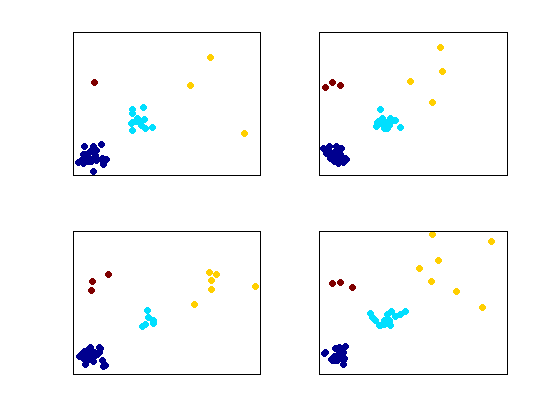
\includegraphics[trim = 4cm 8cm 4cm 8cm, clip, width=4.5cm]{fig/shared_clustering.pdf}
%\caption{Shared clustering}
\label{default}
\end{center}
\end{figure}
\end{column}
\end{columns}
\end{block}
\end{frame}	

\subsection{Pitman-Yor Process}
\frame[t] {
\frametitle{Pitman Yor Process (PYP) : Definition \cite{Pitman1997a}}
 A Pitman-Yor process $\PY(c,d,H)$ is a distribution over distributions with three parameters:
\begin{itemize}
\item A discount $ 0 \le d < 1 $ that controls power-law behavior
\begin{itemize}
\item $d=0$ is DP
\end{itemize}
\item A concentration $c > -d$ like that of the DP
\item A base distribution $H$ also like that of the DP
\end{itemize}
%A draw $G \sim PY(c,d,H)$ is also atomic

%\[G = \sum_{k=1}^{\infty} \pi_k \delta_{\phi_k}\].  
}

\frame[t] {
\frametitle{PYP: Polya Urn Representation}
As in the DP, the PYP posterior predictive distribution can be expressed with $G$ marginalized out.  
\begin{eqnarray*}
p(x_{n+1} | x_{1}, \ldots, x_n) & = & \Ave\left[\frac{m_k - d}{c+n}\delta(\phi_k-\cdot) + \frac{c + Kd}{c + n}H(\cdot)\right]
\end{eqnarray*}

This again forms the basis for similar SMC and MCMC inference algorithms.
\bigskip

%Note: As in the case of the DP, due to the discrete nature of distributions $G \sim \PY(c,d,H)$, draws from $G$ tend to take the same value or ``cluster.''  
}

\frame[t] {
\frametitle{Hierarchical Pitman-Yor Process \cite{Teh2006a}}
A hierarchical Pitman-Yor process is the ``obvious'' two-parameter extension of the hierarchical Dirichlet process \cite{Teh2006b,Goldwater2006}.\\
\bigskip

Example:
%\begin{columns}[t]
%\begin{column}{.75\textwidth}
\begin{eqnarray*}
	\G_{[]} | \U_{\Sigma}, d_0 &\sim& \PY(d_0, 0, \U_{\Sigma }) \\
	\G_{\bf{u}} | \G_{\sigma(\bf{u})}, d_{|\bf{u}|} &\sim& \PY(d_{|\bf{u}|}, 0, \G_{\sigma(\bf{u})}) \hspace{.35cm} \forall {\bf u} \in \Sigma^+\\
	x_n | x_{n-1},  \ldots, x_1 = \bf{u} &\sim& \G_{\bf{u}}
\end{eqnarray*}
%\end{column}
%\begin{column}{.25\textwidth}
%\includegraphics[trim = 4cm 8cm 4cm 8cm, clip, width=5cm]{../../2010_icml/fig/sm_graphical_model.pdf}
%\todo{insert graphical model fig}
%\end{column}
%\end{columns}
%\bigskip
\begin{itemize}
\item Estimation and inference follow that for the hierarchical Dirichlet process (HDP)
\item HDP inference follows closely inference in single level models
\end{itemize}

}

%
\frame[t] {
\frametitle{Pitman Yor Process (PYP) : Definition \cite{Pitman1997a}}
 A Pitman-Yor process $\PY(c,d,H)$ is a distribution over distributions with three parameters:
\begin{itemize}
\item A discount $ 0 \le d < 1 $ that controls power-law behavior
\begin{itemize}
\item $d=0$ is DP
\end{itemize}
\item A concentration $c > -d$ like that of the DP
\item A base distribution $H$ also like that of the DP
\end{itemize}
A draw $G \sim PY(c,d,H)$ is also atomic

\[G = \sum_{k=1}^{\infty} \pi_k \delta_{\phi_k}\].  
}

\frame[t]{
\frametitle{PYP: Stick-Breaking Construction}
The procedure for generating a draw from a PYP is to draw $\pi_k$ from a generalized stick-breaking procedure and $\phi_k$ as usual:
\[
\begin{array}{rcll}
\beta_k  & \sim & \Bet(1-d, c+kd) & \forall \, k = 1 \ldots \infty \\
&&& \\
\pi_k & = &  \beta_k \prod_{i=1}^{k-1}(1- \beta_i) & \forall \, k = 1 \ldots \infty \\
&&& \\
\phi_k  & \sim &  H & \forall \, k = 1 \ldots \infty
\end{array}
\]

The expected length of a stick $\mathbb{E}[\pi_k]$ falls off as a power law for large $k$ when $d \ne 0$.  When $d = 0$ the stick lengths fall off exponentially, and the PYP reduces to a Dirichlet process.
%The expected length of a stick is $\mathbb{E}[\pi_k] = \mathbb{E}[\beta_k]\prod_{i=1}^{k-1}(1 - \mathbb{E}[\beta_i]) = \frac{1-d}{1+c+(k-1)d}\prod_{i=1}^{k-1}\frac{c+id}{1+c+(i-1)d} = d(1-d)\frac{\Gamma(\frac{c}{d} + (k-1))}{\Gamma(\frac{c}{d})}\frac{\Gamma(\frac{1+c}{d})}{\Gamma(\frac{1+c}{d} + k)}$
}

\frame[t] {
\frametitle{PYP: Power Law}
\begin{figure}[t]
\begin{center}
%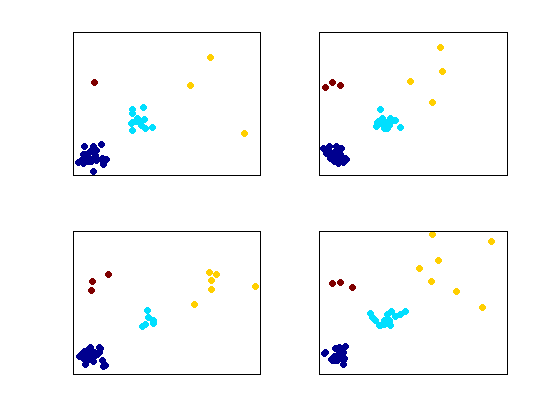
\includegraphics[trim = 4cm 8cm 4cm 8cm, clip, width=5cm]{fig/shared_clustering.pdf}
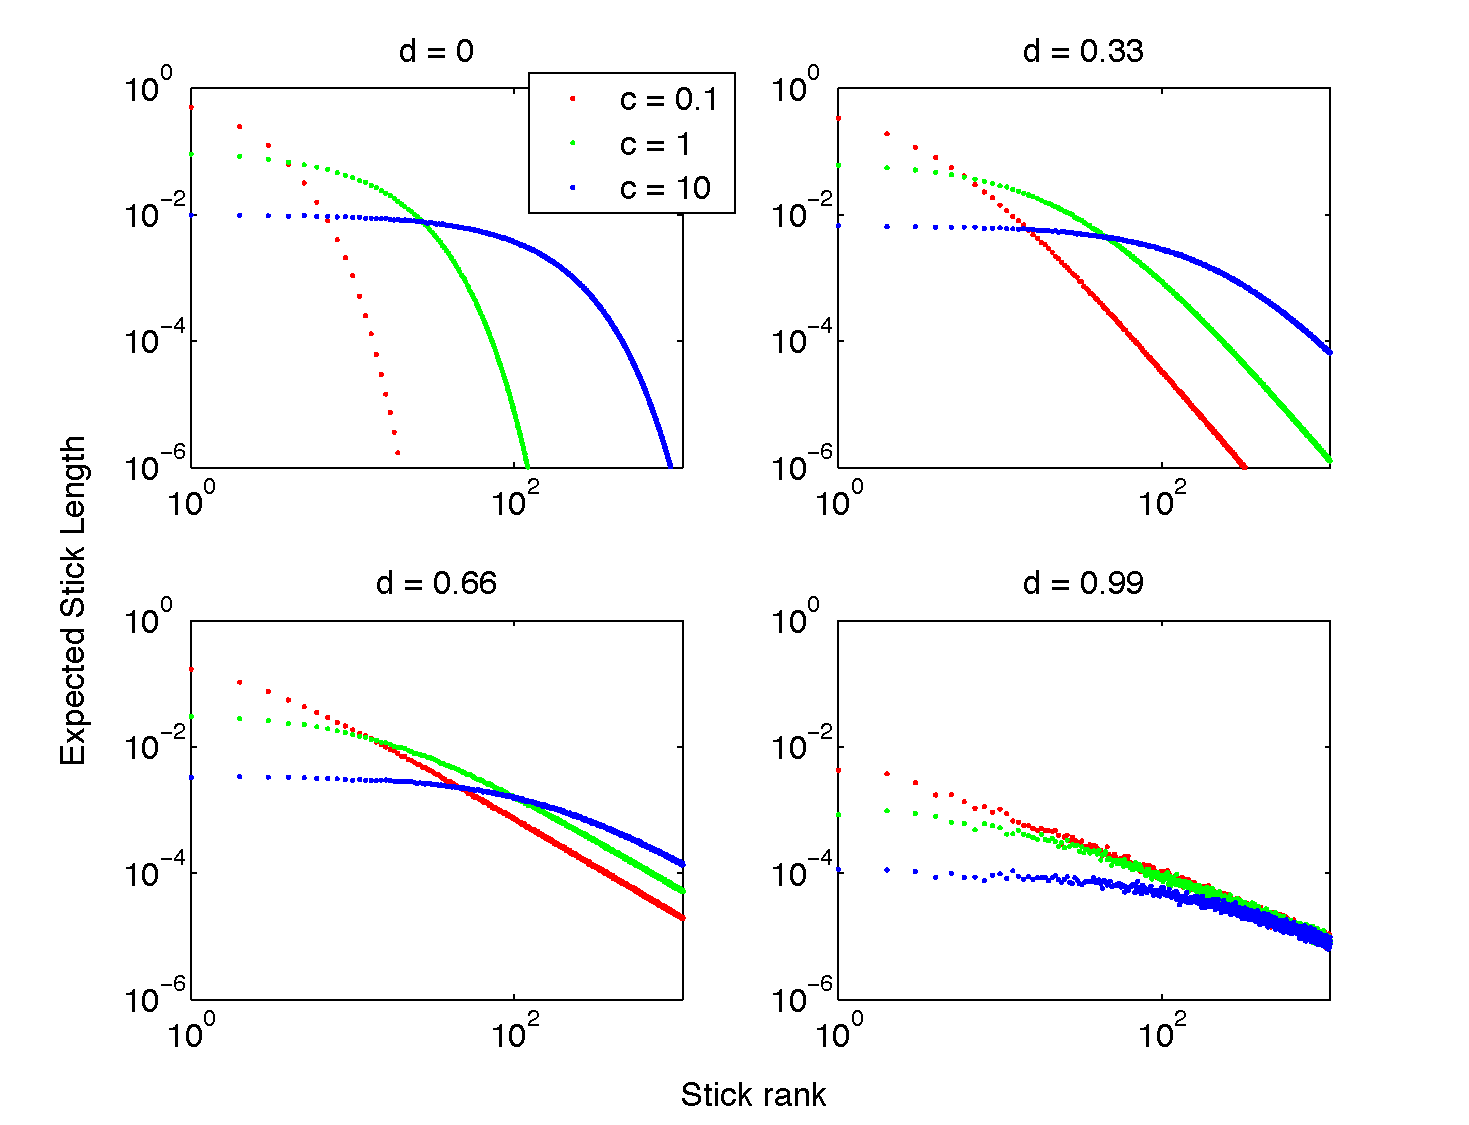
\includegraphics[width=8cm]{jtfig/pypl.pdf}
%\caption{Shared clustering}
\label{default}
\end{center}
\end{figure}
}

\frame[t] {
\frametitle{PYP: Polya Urn Representation}
As in the DP, the PYP posterior predictive distribution can be expressed with $G$ marginalized out.  
\begin{eqnarray*}
p(x_{n+1} | x_{1}, \ldots, x_n) & = & \Ave\left[\frac{m_k - d}{c+n}\delta(\phi_k-\cdot) + \frac{c + Kd}{c + n}H(\cdot)\right]
\end{eqnarray*}

This again forms the basis for similar SMC and MCMC inference algorithms.
\bigskip

Note: As in the case of the DP, due to the discrete nature of distributions $G \sim \PY(c,d,H)$, draws from $G$ tend to take the same value or ``cluster.''  
}

\frame[t] {
\frametitle{Hierarchical Pitman-Yor Process \cite{Teh2006a}}
A hierarchical Pitman-Yor process is the ``obvious'' two-parameter extension of the hierarchical Dirichlet process \cite{Teh2006b,Goldwater2006}.\\
\bigskip

Example:
%\begin{columns}[t]
%\begin{column}{.75\textwidth}
\begin{eqnarray*}
	\G_{[]} | \U_{\Sigma}, d_0 &\sim& \PY(d_0, 0, \U_{\Sigma }) \\
	\G_{\bf{u}} | \G_{\sigma(\bf{u})}, d_{|\bf{u}|} &\sim& \PY(d_{|\bf{u}|}, 0, \G_{\sigma(\bf{u})}) \hspace{.35cm} \forall {\bf u} \in \Sigma^+\\
	x_n | x_{n-1},  \ldots, x_1 = \bf{u} &\sim& \G_{\bf{u}}
\end{eqnarray*}
%\end{column}
%\begin{column}{.25\textwidth}
%\includegraphics[trim = 4cm 8cm 4cm 8cm, clip, width=5cm]{../../2010_icml/fig/sm_graphical_model.pdf}
%\todo{insert graphical model fig}
%\end{column}
%\end{columns}
%\bigskip
Estimation and inference follow that for the hierarchical Dirichlet process
}

\frame[t] {
\frametitle{Review}
\begin{block}{Summary}
\begin{itemize}
\item DP and PYP are flexible priors on distributions
\item Can think of either as glue for tying together related distributions in hierarchical models.
\item 
\end{itemize}
\end{block}
}

%\subsection{Hierarchical Modeling}
%\subsection{Power law}
%\label{powerlaw}

\section{Power Law Processes}

\frame[t] {
\frametitle{Power Law Distribution}
A power law distribution is a distribution whose tail falls off as
\[ P(X=x) \propto x^{-\alpha} \]
For some $\alpha > 1$.  The simplest such distribution is the zeta distribution on natural numbers:
\[ f_\alpha(k) = \frac{k^{-\alpha}}{\zeta(\alpha)} \]
and the Pareto distribution on the real line (with small-scale cutoff $x_{min} > 0$):
\[ f_\alpha(x) = \frac{\alpha-1}{x_{min}} \left(\frac{x}{x_{min}}\right)^{-\alpha} \]
}

\frame[t] {
\frametitle{Scale Free Property}
A power law distribution on the real line is {\em scale free} in the sense that, for all scales $k > 0$ and $x > x_{min}$
\[  f_{\alpha}(kx) \propto f_{\alpha}(x) \]
Where the proportionality constant depends only on $k$.
}

\frame[t] {
\frametitle{Power Laws in Nature}
Words in natural language, arranged by frequency \cite{Zipf1965}.
\begin{center}
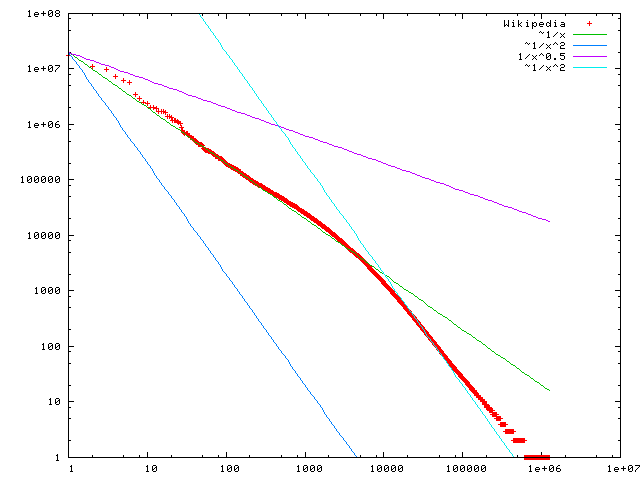
\includegraphics[scale=0.35]{figs/wikipedia-zipf.png} \\
Log-log plot of word frequency in Wikipedia (source: Wikipedia)
\end{center}
}

\frame[t] {
\frametitle{Power Laws in Nature}
Cities arranged by population \cite{Blank2000}.
}

\frame[t] {
\frametitle{Power Laws in Nature}
Earthquakes arranged by magnitude \cite{Gutenberg1955}. \\
\begin{center}
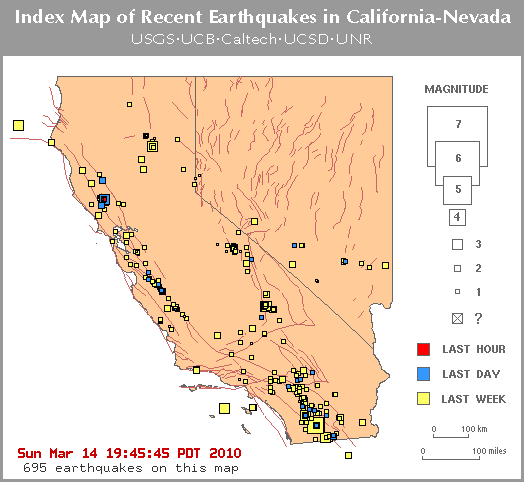
\includegraphics[scale=0.35]{figs/earthquakes.png} \\
(image source: http://quake.usgs.gov/recenteqs/latest.htm)
\end{center}
}

\frame[t] {
\frametitle{Power Laws in Nature}
Power spectra of natural images \cite{Ruderman1994}.
\begin{center}
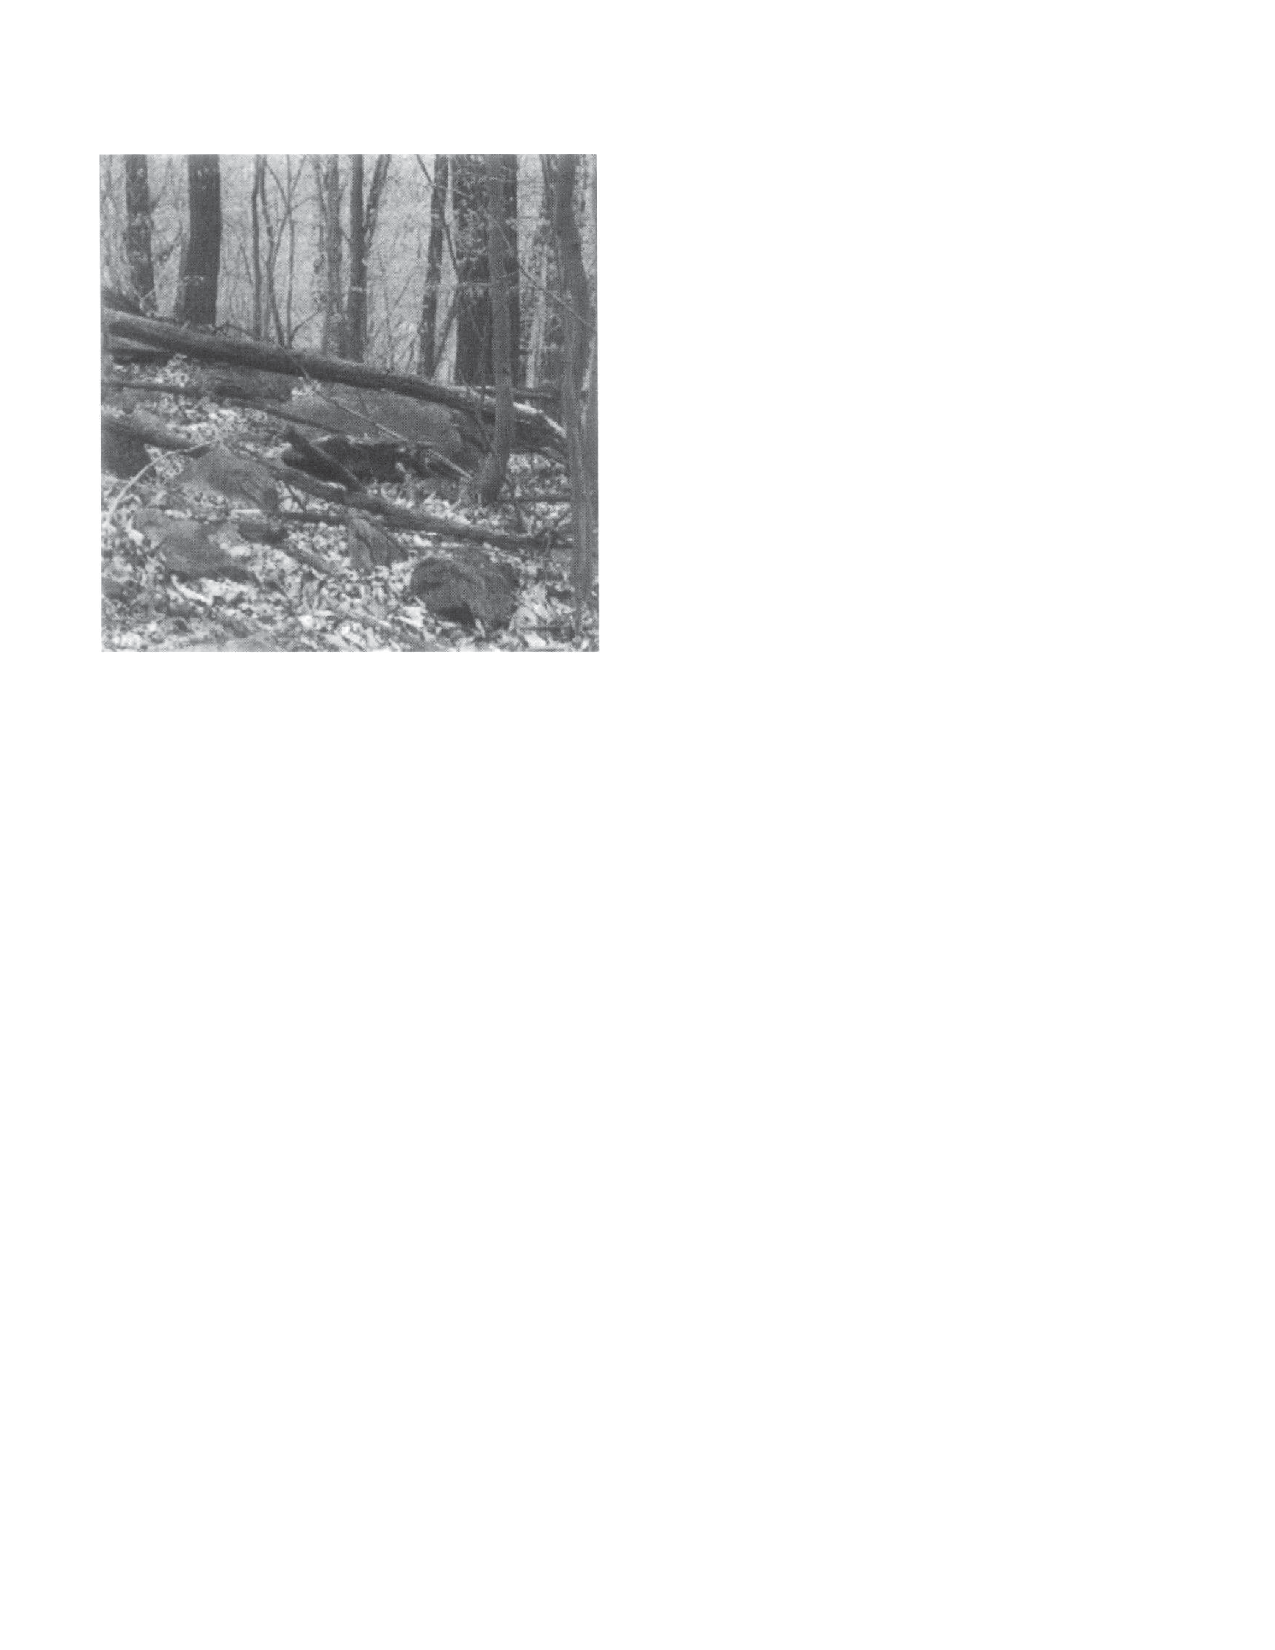
\includegraphics[scale=0.5]{figs/ruderman_bialek_img.pdf}
\hspace*{5 mm}
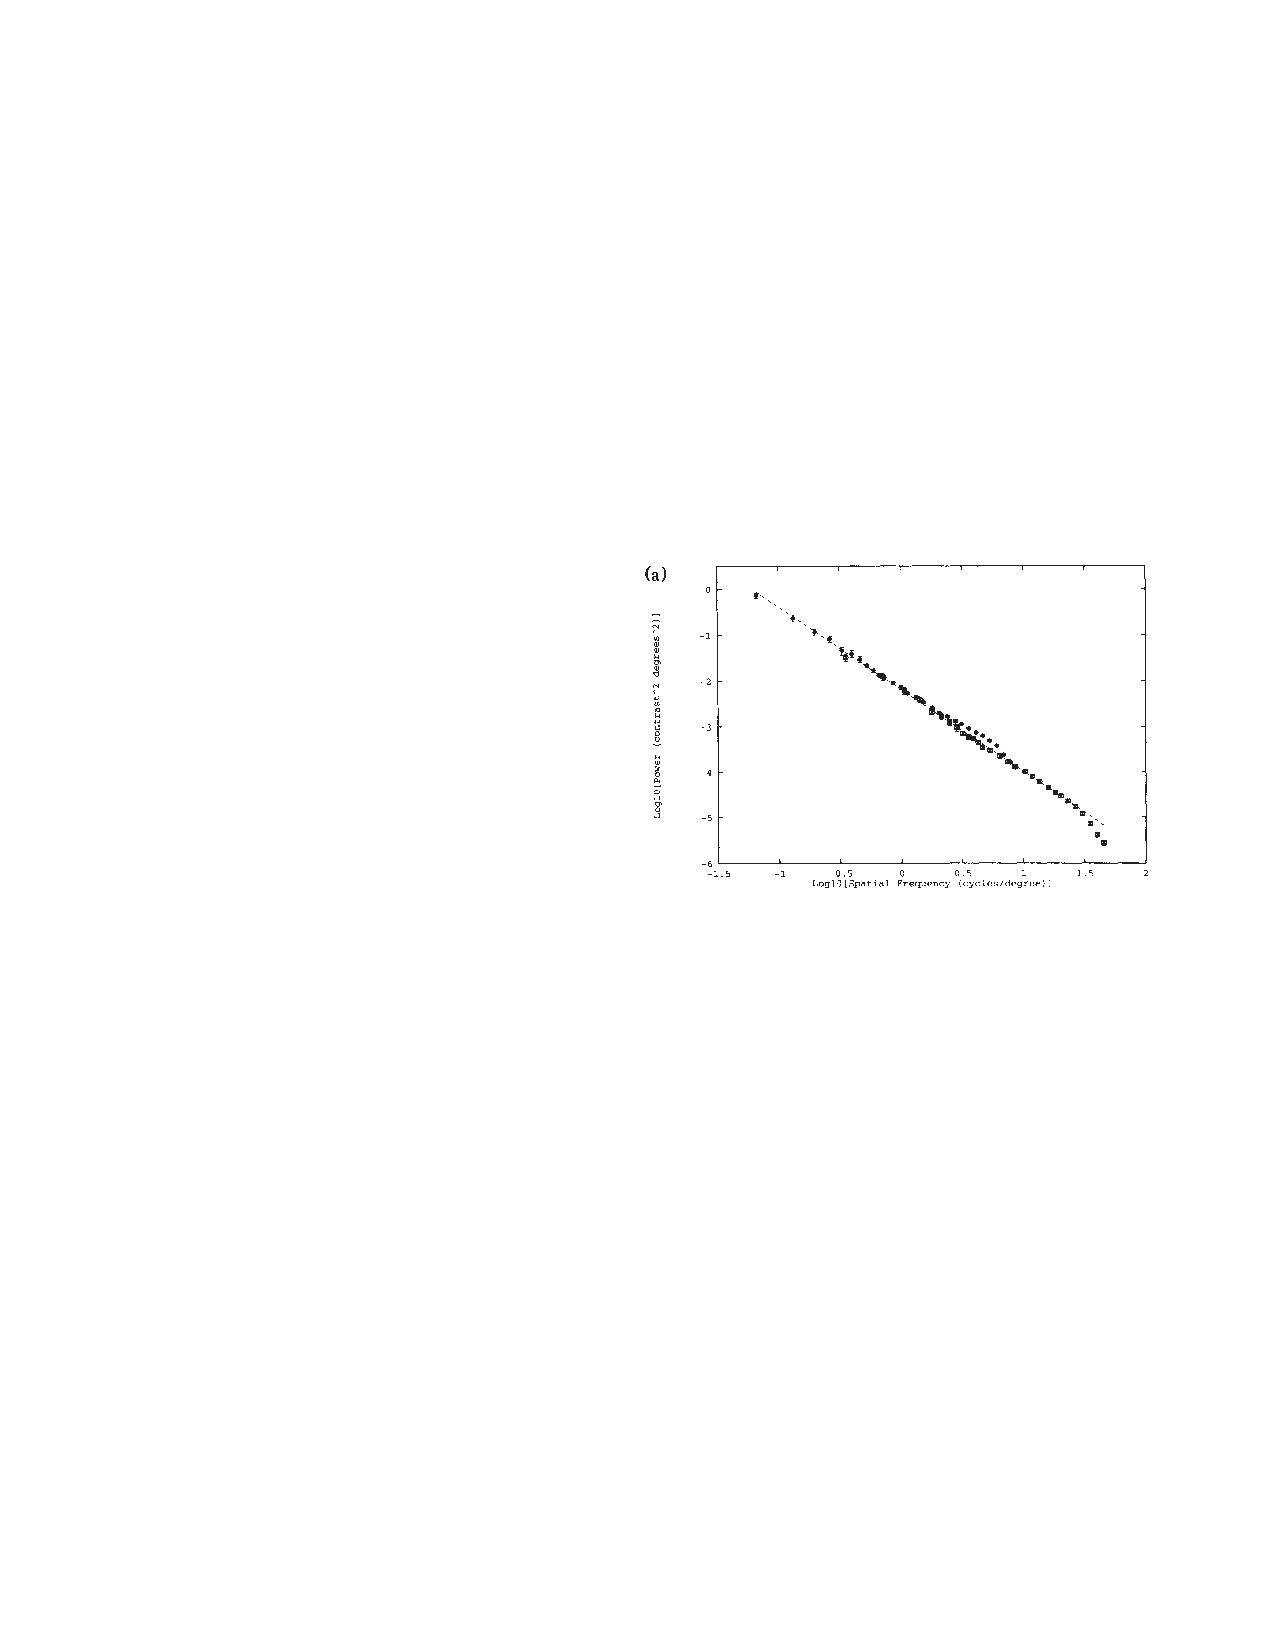
\includegraphics[scale=0.75]{figs/ruderman_bialek_plot.pdf}
\end{center}
}
\section{Sequence Memoizer \hspace{1.5cm}}
\subsection{General Unsupervised Sequence Model}
 \frame[t] {%slide 9
 \frametitle{Big Picture}
 Can we learn a joint distribution of over sequences of unbounded length given a single training sequence? (!!!) \newline
 
\begin{itemize}
\item Obviously not without strong regularization.  
\end{itemize}

 
 \begin{block}{Proposal}
\begin{itemize}
\item Build hierarchical model that ties together conditional distributions in ``natural'' way
\item What would such a model look like?
\end{itemize}
\end{block}
%Let $G_{[\ubf]}$ be the conditional distribution over $\{0,1\}$, conditioned on the binary sequence $\ubf$
}

 \frame[t] {%slide 8
 \frametitle{Regularized Joint Model for Discrete Data}
 Let $\GG = \{G_{[\ubf]}\}, \forall \ubf \in \Sigma^+$ be all conditional distributions over a finite alphabet and $\xbf = x_1, x_2, \ldots, x_n$ be a sequence of discrete observations
\begin{eqnarray*}
P(\xbf,\GG) &=& P(\GG)P(\xbf|\GG) \nonumber \\
P(\xbf,\GG) &=& P(\GG)\prod_{i=0}^{|\xbf|-1}G_{\xbf_{1:i}}(\xbf_{i+1})
\end{eqnarray*}
Where, expanding $P(\xbf|\GG)$ to make it clearer,
\begin{align}
P(\xbf|\GG) = G_{[]}(x_{1})G_{x_1}(x_{2})G_{\xbf_{1:2}}(x_{3})\cdots G_{\xbf_{1:(|\xbf|-1)}}(x_{|\xbf|})  \nonumber 
\end{align}
Note that this is the ``joint''\footnote{$P(x_1,\ldots,x_i|\theta) = P(x_1|\theta) P(x_2 | x_1, \theta) P(x_3 | x_1,x_2, \theta) \cdots P(x_i | \xbf_{1:(i-1)}, \theta)$} distribution of $\xbf$ and $P(\GG)$ directly regularizes the joint distribution itself.

 }




  \frame[t] {%slide 9
 \frametitle{Regularization}
 Bayesian regularization yields posterior inference of the following flavor
 
 \[P(x_{i+1} | \xbf_{1:i}) = \int P(x_{i+1} | \xbf_{1:i}, \GG) dP(\GG | \xbf_{1:i}) \]

where, for DP's and PYP's we can represent and sample directly from $P(x_{i+1} | \xbf_{1:i})$ both individually and in hierarchies, leading to
 \[P(x_{i+1} | \xbf_{1:i}) \approx \frac{1}{L}\sum_{\ell = 1}^L P(x_{i+1} | \xbf_{1:i}, \GG_\ell), \; \GG_\ell \sim P(\GG | \xbf_{1:i})\]

 }




\subsection{Sequence Memoizer}


  \frame[t] {%slide 27
 \frametitle{Sequence Memoizer, \citet{Wood2009}}
\begin{eqnarray*}
\Sigma &=& \{0,1\}\\
\U_{\Sigma } &=& [.5, .5] \\
\\
	\G_{[]} | \U_{\Sigma}, d_0 &\sim& \PY(d_0, 0, \U_{\Sigma }) \\
		\G_{\bf{u}} | \G_{\sigma(\bf{u})}, d_{|\bf{u}|} &\sim& \PY(d_{|\bf{u}|}, 0, \G_{\sigma(\bf{u})}) \hspace{.35cm} \forall {\bf u} \in \Sigma^+\\
	x_n | x_{n-1},  \ldots, x_1 = \bf{u} &\sim& \G_{\bf{u}}
\end{eqnarray*}
Here $\sigma(x_1x_2x_3\ldots x_n) = x_2x_3\ldots x_n$ is the suffix operator.
\bigskip
\begin{center}
We're done, right?
\end{center}
}

  \frame[t] {%slide 27
 \frametitle{A Way to Tie Together ``Related'' Conditional Distributions}
 \begin{figure}[htbp]
\begin{center}
%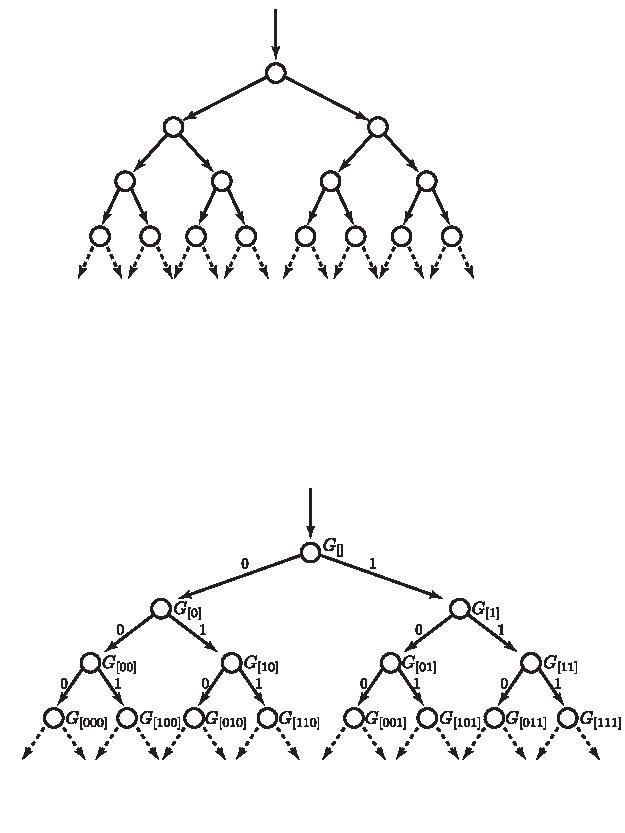
\includegraphics[trim = 4cm 8cm 4cm 8cm, clip, width=5cm]{jtfig/base.pdf}
\vspace{2cm}
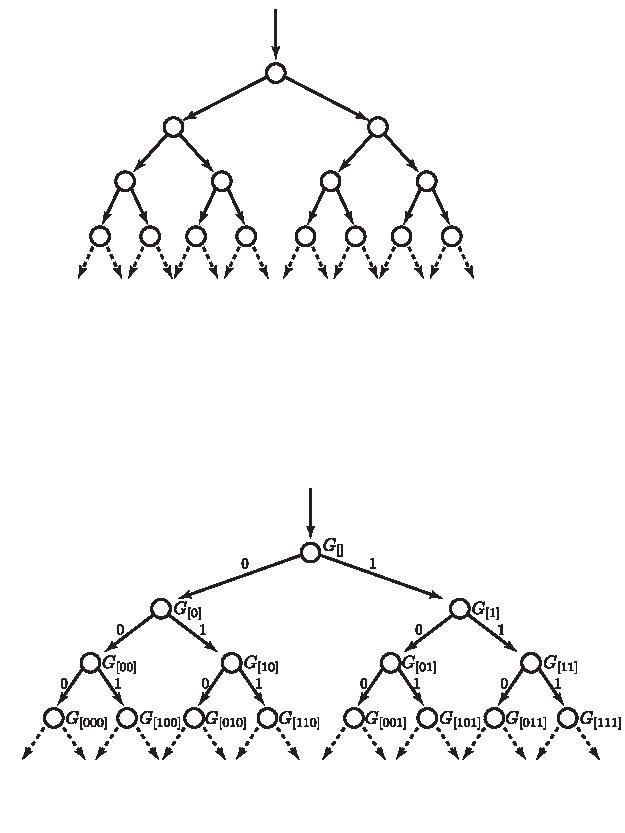
\includegraphics[trim = 2cm 2cm 2cm 10cm, width=8cm]{jtfig/base.pdf}
%\caption{Test perplexity vs.~number of training observations.}
\label{fig: gm_binary_complete}
\end{center}
\end{figure}
}

\comment{
\begin{frame}[t]{Computational Problems}
\begin{itemize}
\item Number of nodes in graphical model is $\mathcal{O}(2^n)$
\begin{itemize}
\item Solution : marginalize (ignore) conditional distributions not found in sequence
\end{itemize}
\item Number of conditional distributions in graphical model still grows $\mathcal{O}(n^2)$
\begin{itemize}
\item Solution, \citet{Wood2009} : marginalize out non-branching nodes \cite{Pitman1999, Ho2006}
\item Use suffix tree algorithms to identify  $\mathcal{O}(n)$ remaining nodes.
\end{itemize}
\item Number of conditional distributions grows as $\mathcal{O}(n)$ but suffix tree algorithms require full sequence
\begin{itemize}
\item Solution, \citet{Gasthaus2010} : note (worst-case) $\mathcal{O}(n^2)$ inference time and show that incremental construction algorithm suffices
\end{itemize}
\item Number of nodes grows as $\mathcal{O}(n)$
\begin{itemize}
\item Solution, \citet{Bartlett2010} : forget nodes 
\end{itemize}
\end{itemize}
\end{frame}
}





 \begin{frame}[t]{Computational Problems}
\begin{itemize}
\item Number of nodes in graphical model is $\mathcal{O}(2^n)$
\begin{itemize}
\item Solution : marginalize (ignore) conditional distributions not found in sequence
\end{itemize}
\end{itemize}
\end{frame}
  
 
 
  \frame[t] {%slide 27
 \frametitle{Graphical Model}
 \begin{figure}[htbp]
\begin{center}
%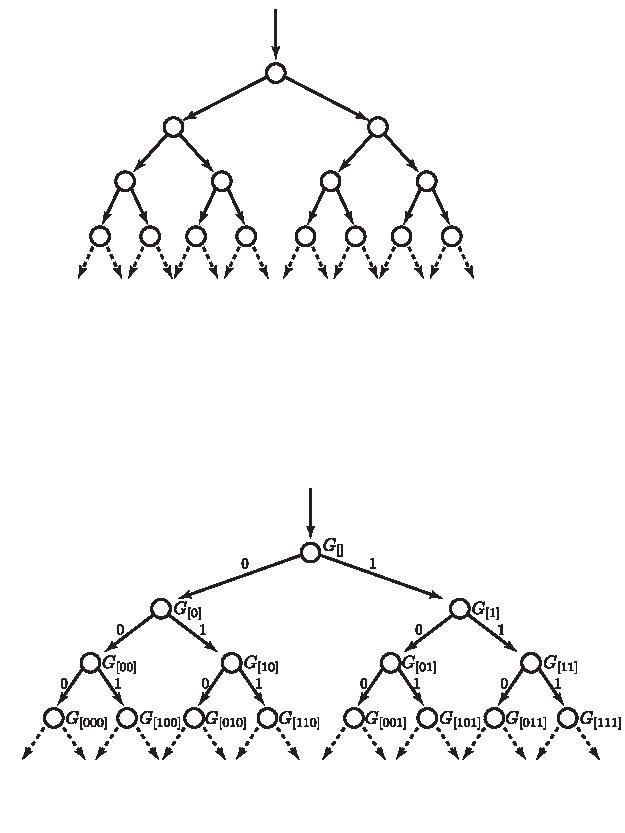
\includegraphics[trim = 4cm 8cm 4cm 8cm, clip, width=5cm]{jtfig/base.pdf}
\vspace{2cm}
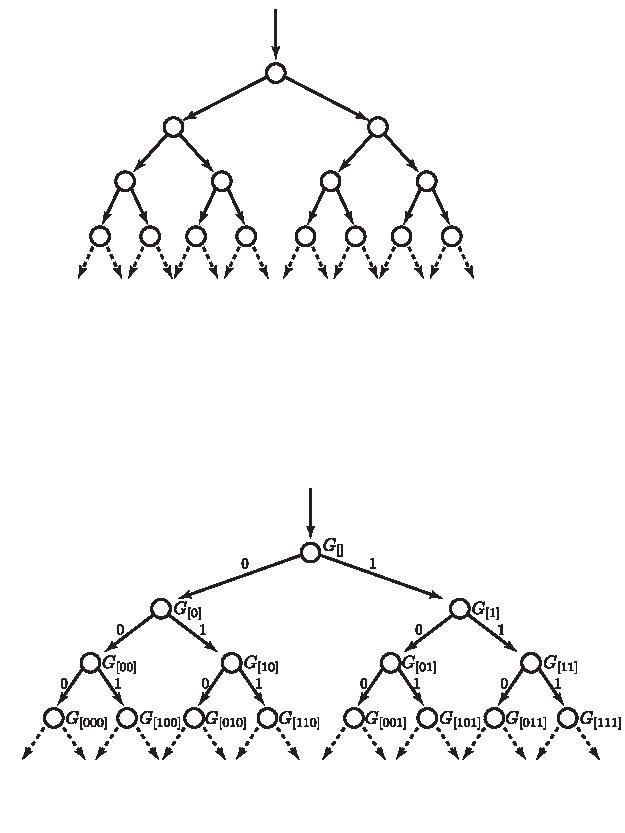
\includegraphics[trim = 2cm 2cm 2cm 10cm, width=8cm]{jtfig/base.pdf}
%\caption{Test perplexity vs.~number of training observations.}
\label{fig: gm_binary_complete}
\end{center}
\end{figure}
}

  \frame[t] {%slide 27
 \frametitle{110100, $G_{[]}(1)G_{[1]}(1)G_{[11]}(0)G_{[110]}(1)G_{[1101]}(0)G_{[11010]}(0)$}
 \begin{figure}[htbp]
\begin{center}
%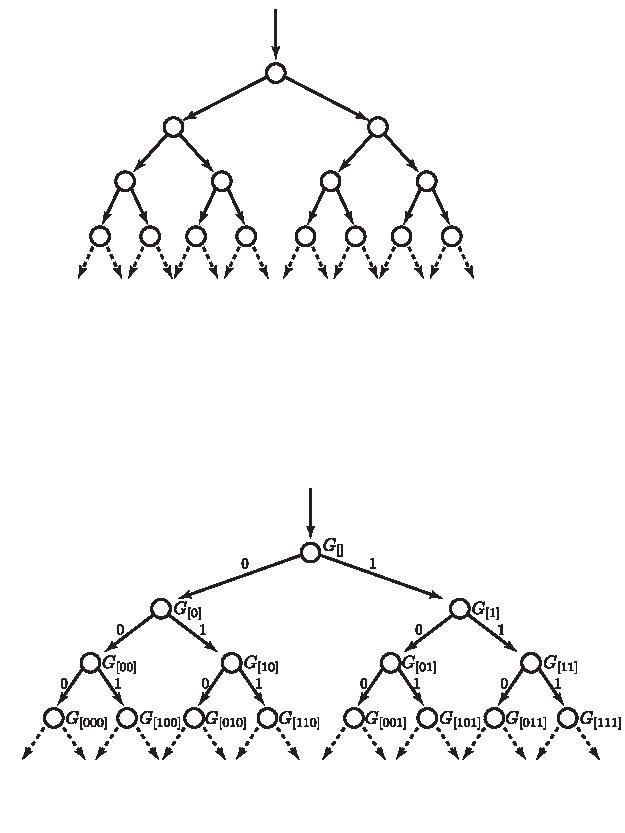
\includegraphics[trim = 4cm 8cm 4cm 8cm, clip, width=5cm]{jtfig/base.pdf}
\vspace{.42cm}
\hspace{.42cm}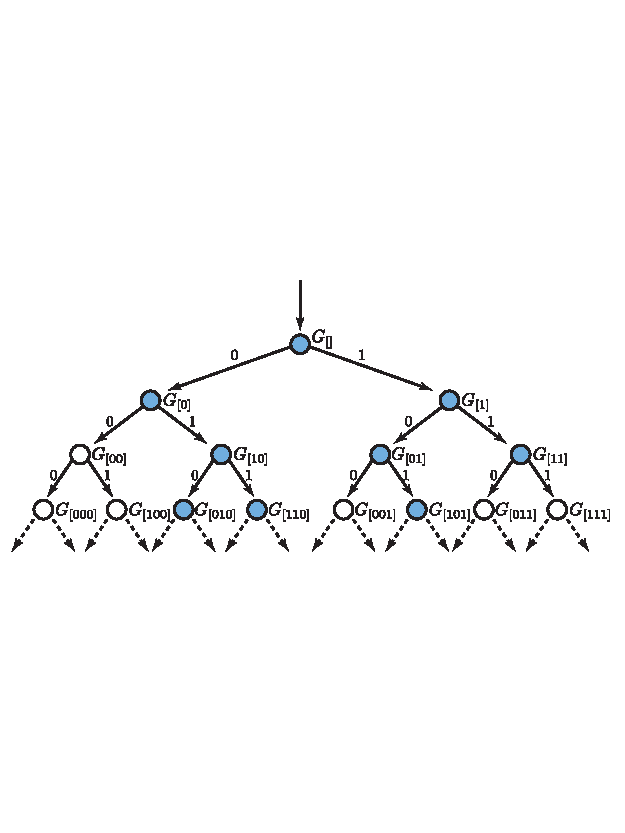
\includegraphics[trim = 2cm 2cm 2cm 5cm, width=8cm]{jtfig/base_color_2.pdf}
%\caption{Test perplexity vs.~number of training observations.}
\label{fig: gm_binary_complete}
\end{center}
\end{figure}
}

\begin{frame}[t]{Computational Problems}
\begin{itemize}
\item Number of nodes in graphical model is $\mathcal{O}(2^n)$
\begin{itemize}
\item Solution : marginalize (ignore) conditional distributions not found in sequence
\end{itemize}
\item Number of conditional distributions in graphical model still grows $\mathcal{O}(n^2)$
\begin{itemize}
\item Solution, \citet{Wood2009} : marginalize out non-branching nodes \cite{Pitman1999, Ho2006}
\item Use suffix tree algorithms to identify  $\mathcal{O}(n)$ remaining nodes.
\end{itemize}
\end{itemize}
\end{frame}



 \frame[t] {%slide 27
 \frametitle{Coagulation}
Consider a single path in the graphical model, say \[G_1\rightarrow G_2\rightarrow G_3\] with $G_2$ having no children other than $G_3$.    
\begin{block}{Theorem : Coagulation \cite{Pitman1999, Ho2006}}
If \[G_2| G_1\sim\py(d_1,0,G_1)\] and \[G_3| G_2\sim\py(d_2,0,G_2)\] then
\[G_3|G_1\sim\py(d_1d_2,0,G_1)\] with $G_2$ marginalized out.
\label{thm:coag}
\end{block}
Marginalizing out $G_2$ leaves $G_1\rightarrow G_3$ within the same PY family.

 }

 \frame[t] {%slide 27
 \frametitle{Graphical Model for 110100}
 \begin{figure}[htbp]
\begin{center}
%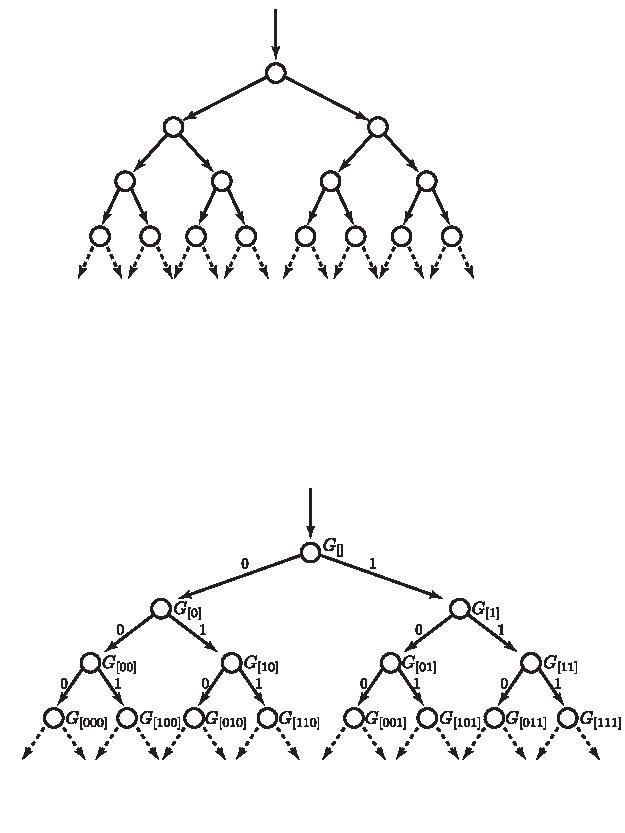
\includegraphics[trim = 4cm 8cm 4cm 8cm, clip, width=5cm]{jtfig/base.pdf}
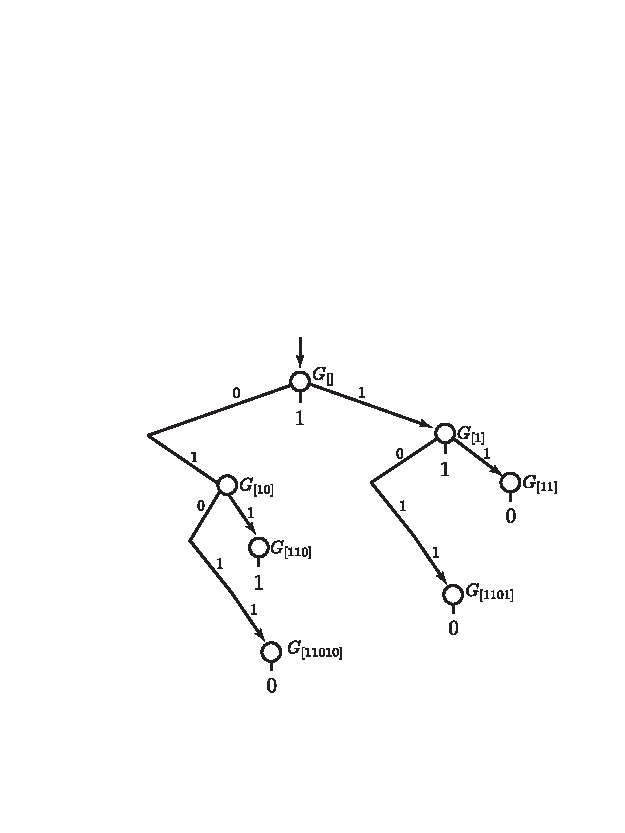
\includegraphics[trim = 2cm 2cm 2cm 6cm, width=8cm]{jtfig/seq_6.pdf}
%\caption{Test perplexity vs.~number of training observations.}
\label{fig: gm_binary_complete}
\end{center}
\end{figure}

 }

 \frame[t] {%slide 27
 \frametitle{Complete Graphical Model with 110100 Subset Highlighted}
 \begin{figure}[htbp]
\begin{center}
%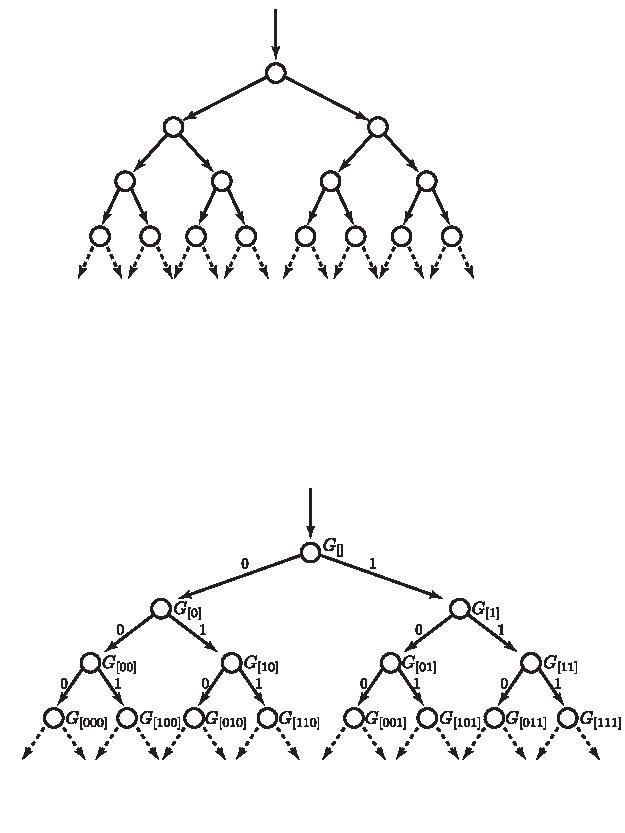
\includegraphics[trim = 4cm 8cm 4cm 8cm, clip, width=5cm]{jtfig/base.pdf}
\vspace{.42cm}
\hspace{.42cm}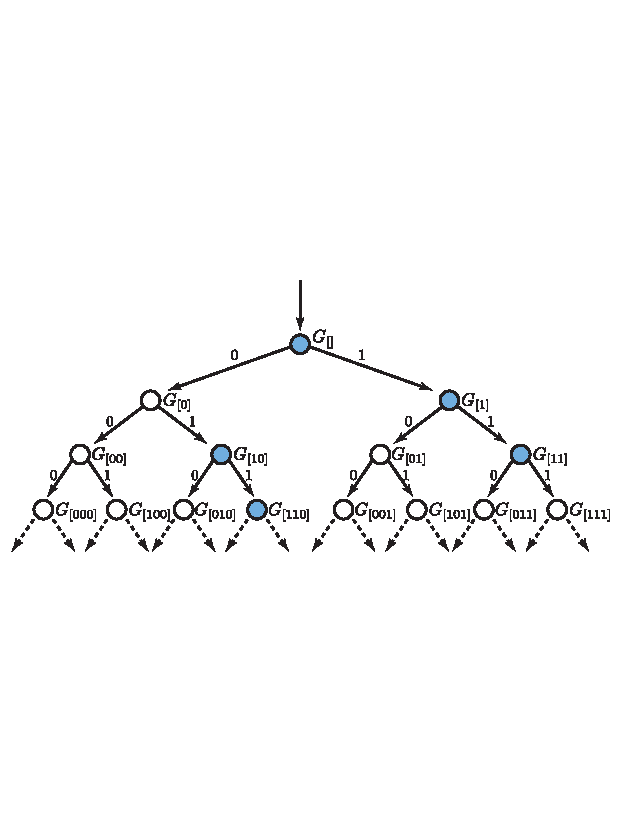
\includegraphics[trim = 2cm 2cm 2cm 5cm, width=8cm]{jtfig/base_color_1.pdf}
%\caption{Test perplexity vs.~number of training observations.}
\label{fig: gm_binary_complete}
\end{center}
\end{figure}
}

\begin{frame}[t]{Computational Problems}
\begin{itemize}
\item Number of nodes in graphical model is $\mathcal{O}(2^n)$
\begin{itemize}
\item Solution : marginalize (ignore) conditional distributions not found in sequence
\end{itemize}
\item Number of conditional distributions in graphical model still grows $\mathcal{O}(n^2)$
\begin{itemize}
\item Solution, \citet{Wood2009} : marginalize out non-branching nodes \cite{Pitman1999, Ho2006}
\item Use suffix tree algorithms to identify  $\mathcal{O}(n)$ remaining nodes.
\end{itemize}
\item Number of conditional distributions grows as $\mathcal{O}(n)$ but suffix tree algorithms require full sequence
\begin{itemize}
\item Solution, \citet{Gasthaus2010} : note (worst-case) $\mathcal{O}(n^2)$ inference time and show that incremental construction algorithm suffices
\end{itemize}
\end{itemize}
\end{frame}

  \frame[t] {%slide 27
 \frametitle{Graphical Model for 110100}
 \begin{figure}[htbp]
\begin{center}
%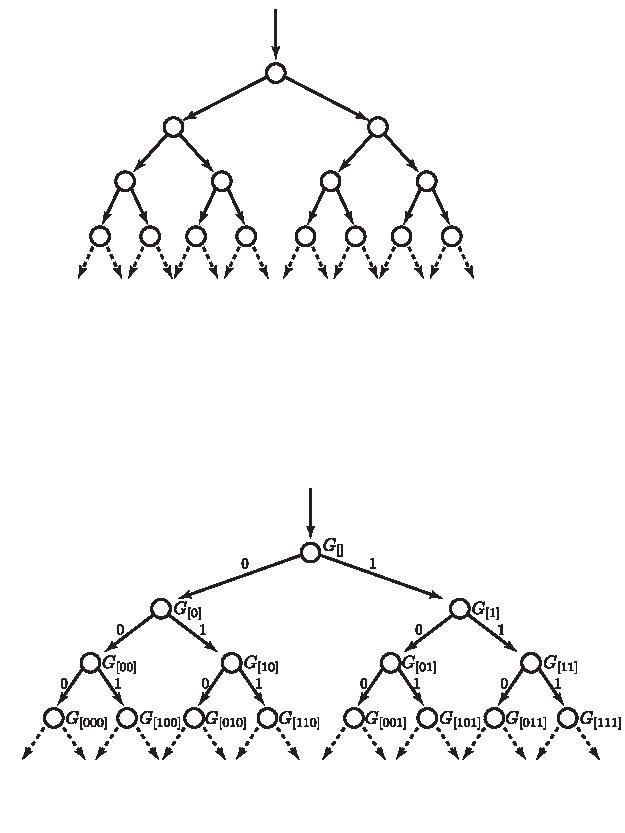
\includegraphics[trim = 4cm 8cm 4cm 8cm, clip, width=5cm]{jtfig/base.pdf}
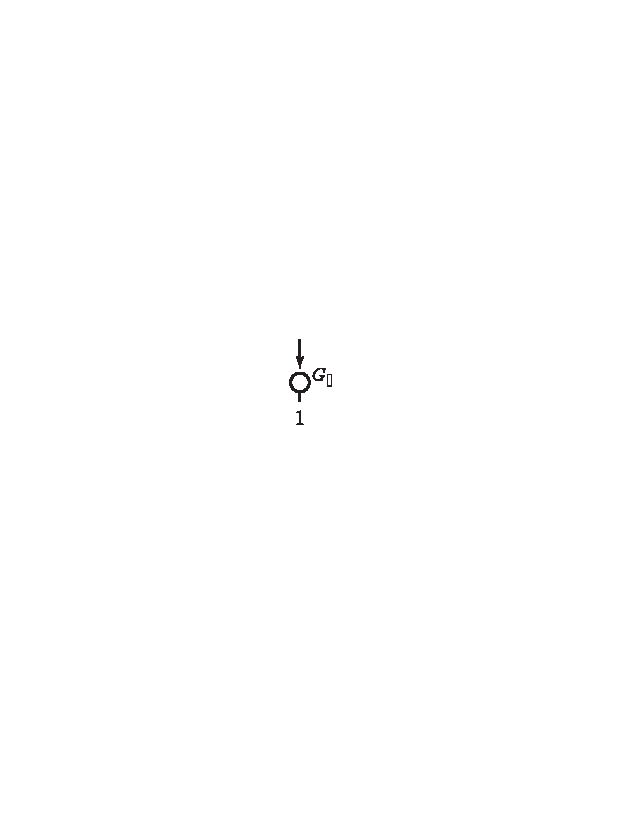
\includegraphics[trim = 2cm 2cm 2cm 6cm, width=8cm]{jtfig/seq_1.pdf}
%\caption{Test perplexity vs.~number of training observations.}
\label{fig: gm_binary_complete}
\end{center}
\end{figure}

 }
 
   \frame[t] {%slide 27
 \frametitle{Graphical Model for 110100}
 \begin{figure}[htbp]
\begin{center}
%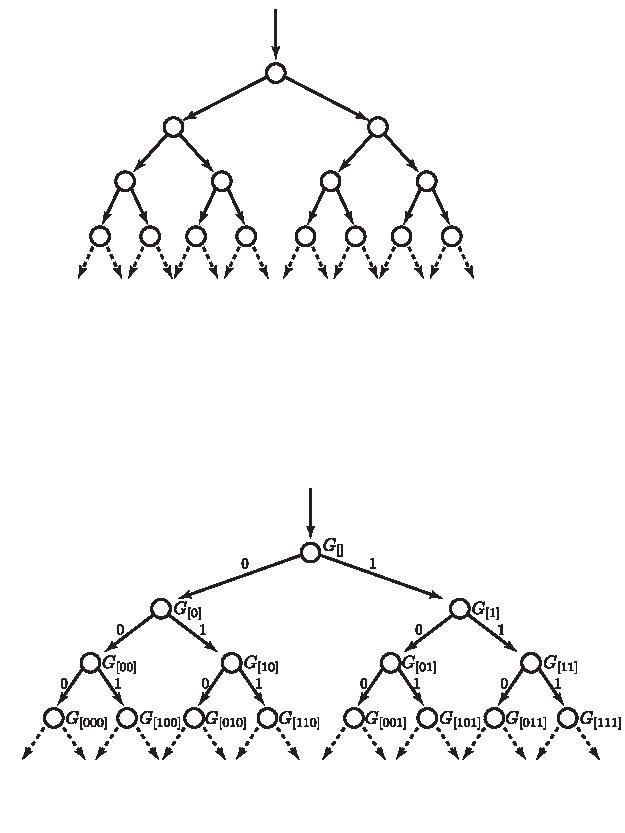
\includegraphics[trim = 4cm 8cm 4cm 8cm, clip, width=5cm]{jtfig/base.pdf}
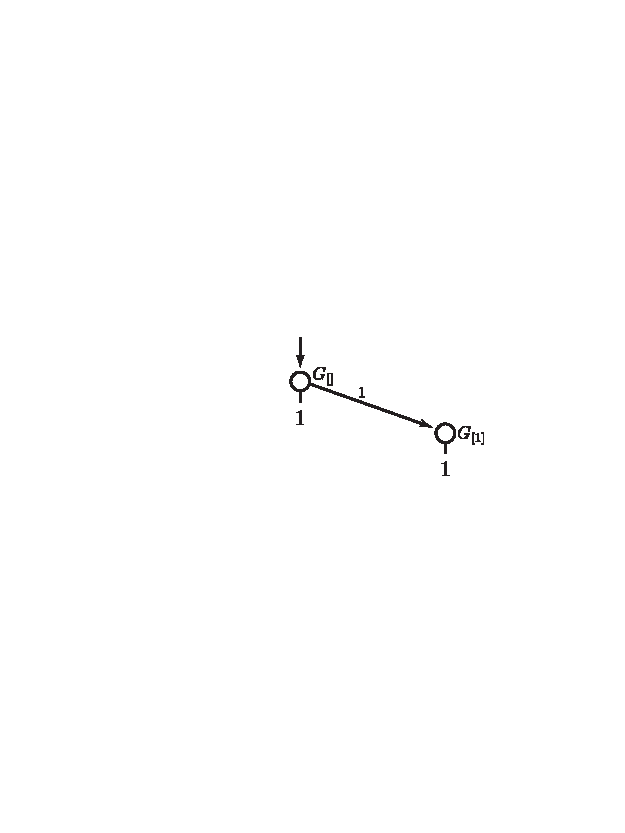
\includegraphics[trim = 2cm 2cm 2cm 6cm, width=8cm]{jtfig/seq_2.pdf}
%\caption{Test perplexity vs.~number of training observations.}
\label{fig: gm_binary_complete}
\end{center}
\end{figure}

 }

  \frame[t] {%slide 27
 \frametitle{Graphical Model for 110100}
 \begin{figure}[htbp]
\begin{center}
%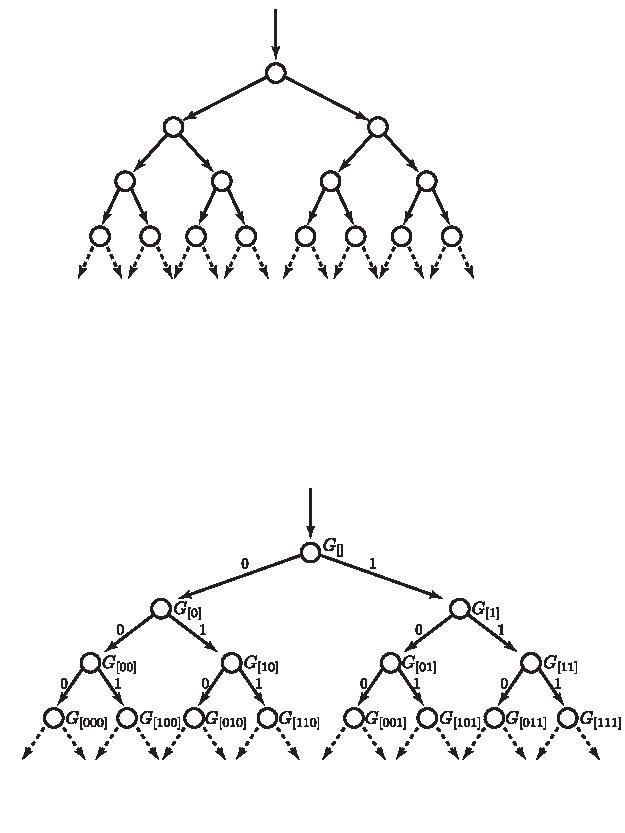
\includegraphics[trim = 4cm 8cm 4cm 8cm, clip, width=5cm]{jtfig/base.pdf}
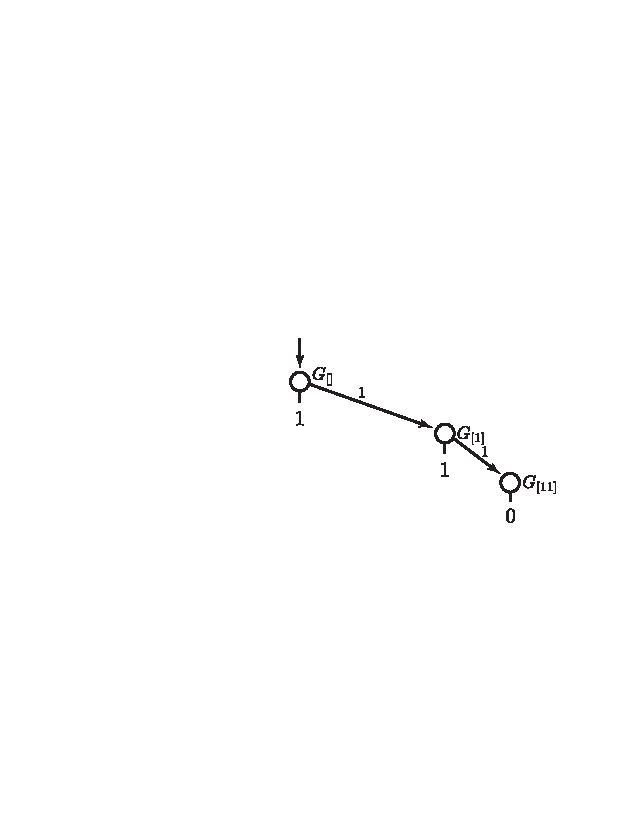
\includegraphics[trim = 2cm 2cm 2cm 6cm, width=8cm]{jtfig/seq_3.pdf}
%\caption{Test perplexity vs.~number of training observations.}
\label{fig: gm_binary_complete}
\end{center}
\end{figure}

 }
   \frame[t] {%slide 27
 \frametitle{Graphical Model for 110100}
 \begin{figure}[htbp]
\begin{center}
%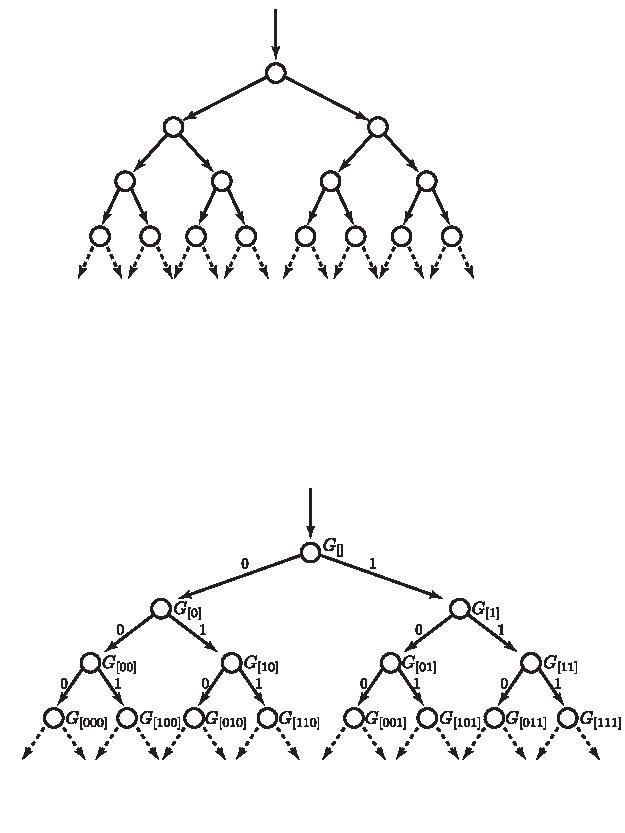
\includegraphics[trim = 4cm 8cm 4cm 8cm, clip, width=5cm]{jtfig/base.pdf}
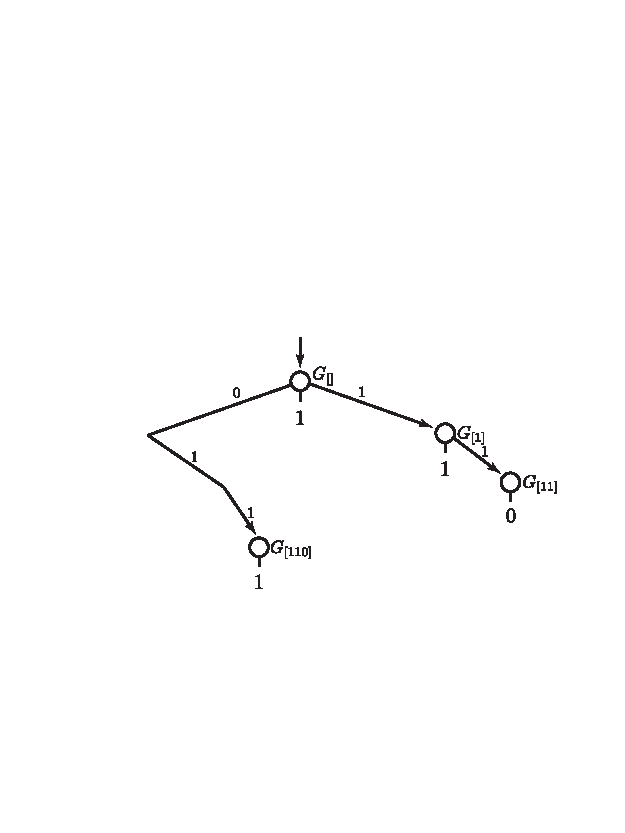
\includegraphics[trim = 2cm 2cm 2cm 6cm, width=8cm]{jtfig/seq_4.pdf}
%\caption{Test perplexity vs.~number of training observations.}
\label{fig: gm_binary_complete}
\end{center}
\end{figure}

 }
   \frame[t] {%slide 27
 \frametitle{Graphical Model for 110100}
 \begin{figure}[htbp]
\begin{center}
%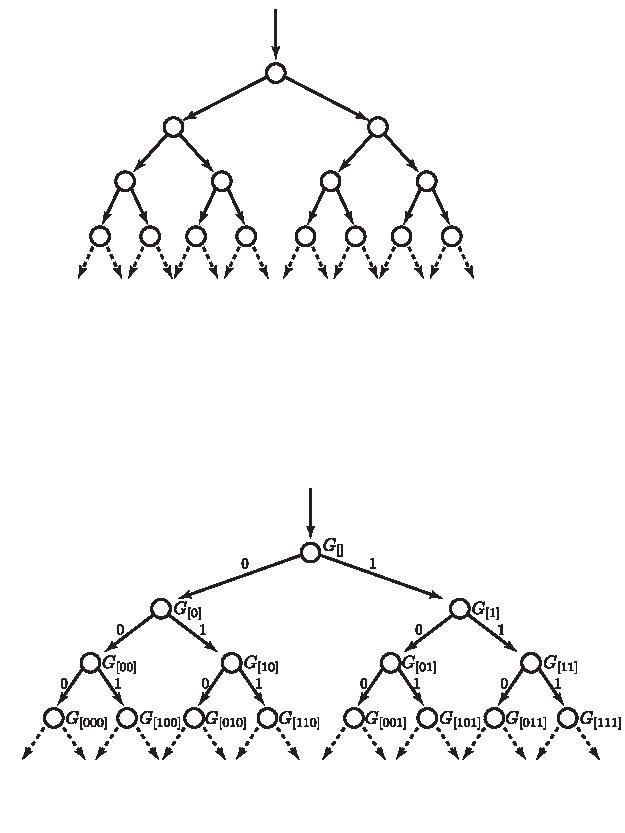
\includegraphics[trim = 4cm 8cm 4cm 8cm, clip, width=5cm]{jtfig/base.pdf}
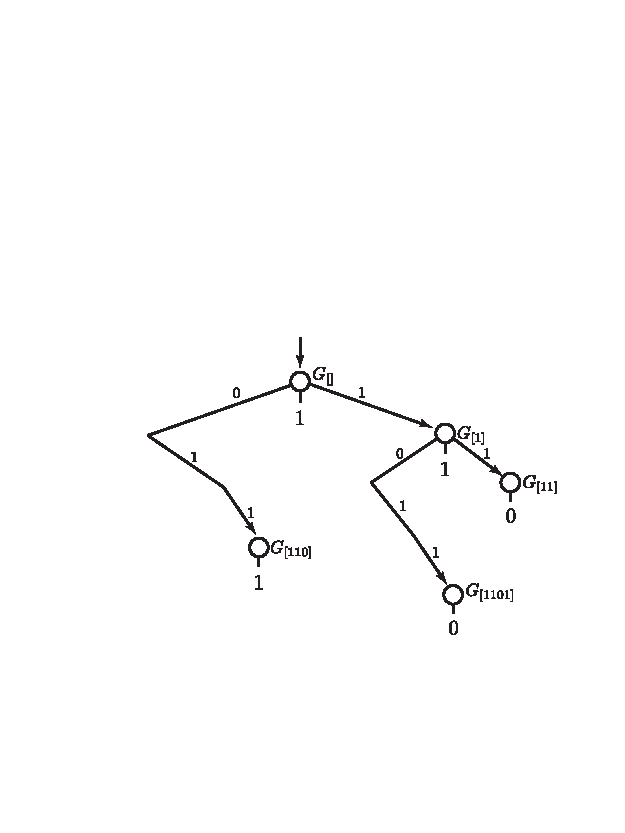
\includegraphics[trim = 2cm 2cm 2cm 6cm, width=8cm]{jtfig/seq_5.pdf}
%\caption{Test perplexity vs.~number of training observations.}
\label{fig: gm_binary_complete}
\end{center}
\end{figure}

 }
   \frame[t] {%slide 27
 \frametitle{Graphical Model for 110100}
 \begin{figure}[htbp]
\begin{center}
%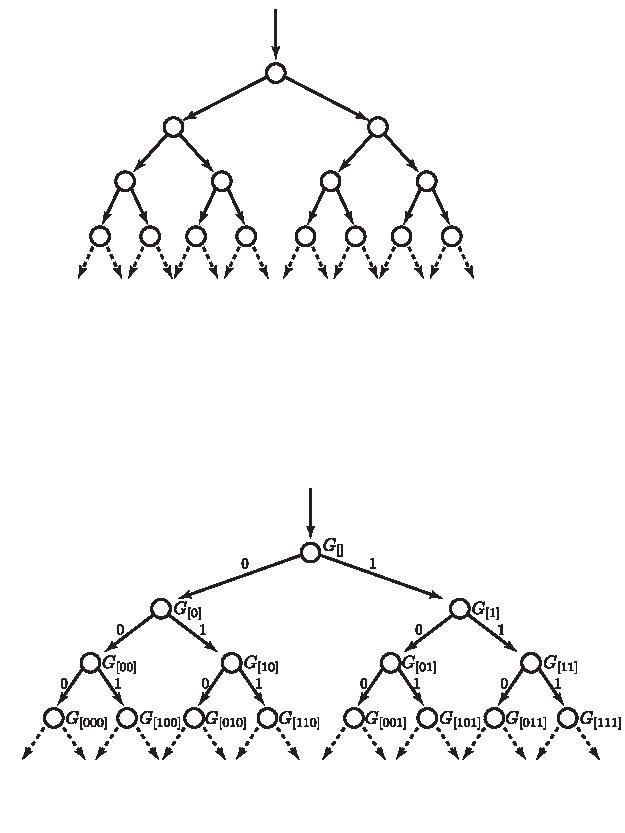
\includegraphics[trim = 4cm 8cm 4cm 8cm, clip, width=5cm]{jtfig/base.pdf}
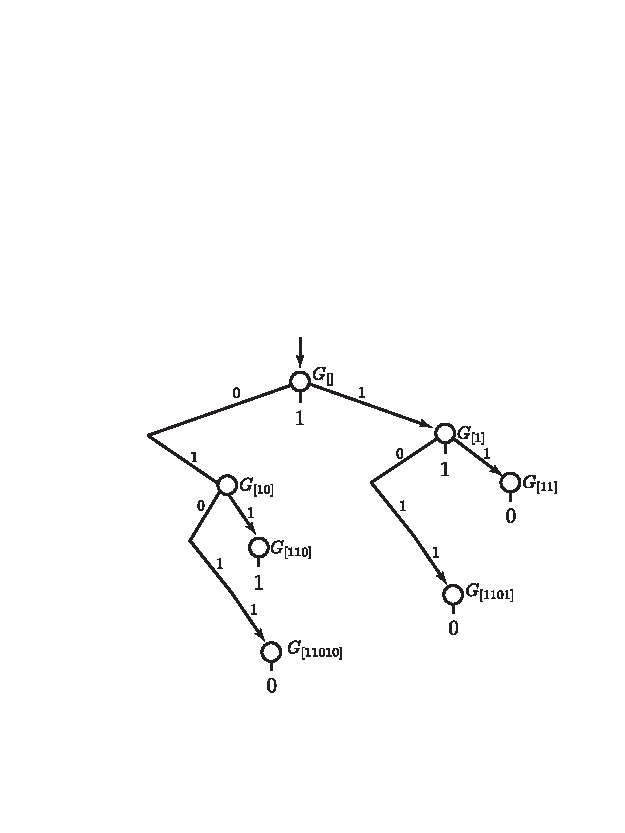
\includegraphics[trim = 2cm 2cm 2cm 6cm, width=8cm]{jtfig/seq_6.pdf}
%\caption{Test perplexity vs.~number of training observations.}
\label{fig: gm_binary_complete}
\end{center}
\end{figure}

 }
 
 \begin{frame}[t]{Computational Problems}
\begin{itemize}
\item Number of nodes in graphical model is $\mathcal{O}(2^n)$
\begin{itemize}
\item Solution : marginalize (ignore) conditional distributions not found in sequence
\end{itemize}
\item Number of conditional distributions in graphical model still grows $\mathcal{O}(n^2)$
\begin{itemize}
\item Solution, \citet{Wood2009} : marginalize out non-branching nodes \cite{Pitman1999, Ho2006}
\item Use suffix tree algorithms to identify  $\mathcal{O}(n)$ remaining nodes.
\end{itemize}
\item Number of conditional distributions grows as $\mathcal{O}(n)$ but suffix tree algorithms require full sequence
\begin{itemize}
\item Solution, \citet{Gasthaus2010} : note (worst-case) $\mathcal{O}(n^2)$ inference time and show that incremental construction algorithm suffices
\end{itemize}
\item Number of nodes grows as $\mathcal{O}(n)$
\begin{itemize}
\item Solution, \citet{Bartlett2010} : forget nodes 
\end{itemize}
\end{itemize}
\end{frame}

 \frame[t] {%slide 24
 \frametitle{Forgetting}
\begin{itemize}
\item Unit of memory is node in graphical model.  
\item Randomly removing leaf nodes defines a ``dependent hierarchical Pitman Yor process'' 
\item Incremental inference in this model is possible
\item The resulting model has constant storage complexity.
\end{itemize}
 }

 
 
 

\section{Demonstration}
\subsection{Lossless compression}
\frame[t] {%slide 2
 \frametitle{Review}
\begin{block}{Shannon's source coding theorem}
$n$ i.i.d. random variables each with entropy $H(\mathcal{X})$ can be compressed into more than $nH(\mathcal{X})$ bits with negligible risk of information loss, as $n$ tends to infinity; but conversely, if they are compressed into fewer than $nH(\mathcal{X})$ bits it is virtually certain that information will be lost. \cite{MacKay2003}
\end{block}
Arithmetic and range coding achieve this limit for all practical purposes.
\bigskip

This means that a lossless compressor built on a sequence predictor will achieve a compression rate equal to the average predictive log-loss, $\ell(\xbf_{1:N}) = -\frac{1}{N}\sum_{i=1}^N \log_2 P(x_i|\xbf_{1:i-1})$
 }
 
{\tiny \frame[t]{
\frametitle{Compression Based on the Incremental Sequence Memoizer}
\begin{table}[t]
    \begin{center}
    \setlength{\tabcolsep}{1.3mm}
\begin{tabular}{|l|r||c|c|c|c||c|c|c|c||c|c|}
\hline
\multicolumn{2}{|c||}{} & \multicolumn{2}{c||}{DEPLUMP} &
\multicolumn{2}{|c|}{PPM} & CTW\\\hline
File          &  Size  &    1PF    &    UKN    &   PPM* &    PPMZ  &  CTW  \\\hline 
\hline
bib           & 111261 &    1.73   &\alert{1.72}  &   1.91 &    1.74  &  1.83 \\\hline
book1         & 768771 &\alert{2.17}  &    2.20   &   2.40 &    2.21  &  2.18 \\\hline
book2         & 610856 &\alert{1.83}  &    1.84   &   2.02 &    1.87  &  1.89 \\\hline
geo           & 102400 &\alert{4.40}  &    4.40   &   4.83 &    4.64  &  4.53 \\\hline
news          & 377109 &\alert{2.20}  &    2.20   &   2.42 &    2.24  &  2.35 \\\hline
obj1          & 21504  &\alert{3.64}  &    3.65   &   4.00 &    3.66  &  3.72 \\\hline
obj2          & 246814 &    2.21   &\alert{2.19}  &   2.43 &    2.23  &  2.40 \\\hline
paper1        & 53161  &    2.21   &\alert{2.20}  &   2.37 &    2.22  &  2.29 \\\hline
paper2        & 82199  &\alert{2.18}  &    2.18   &   2.36 &    2.21  &  2.23 \\\hline
pic           & 513216 &    0.77   &    0.82   &   0.85 &\alert{0.76} &  0.80 \\\hline
progc         & 39611  &    2.23   &\alert{2.21}  &   2.40 &    2.25  &  2.33 \\\hline
progl         & 71646  &    1.44   &\alert{1.43}  &   1.67 &    1.46  &  1.65 \\\hline
progp         & 49379  &    1.44   &\alert{1.42}  &   1.62 &    1.47  &  1.68 \\\hline
trans         & 93695  &    1.21   &\alert{1.20}  &   1.45 &    1.23  &  1.44 \\\hline \hline
\textbf{avg.} &        &\alert{2.12}  &    2.12   &   2.34 &    2.16  &  2.24 \\\hline
\textbf{w.~avg.} &     &\alert{1.89}  &    1.91   &   2.09 &    1.93  &  1.99 \\\hline
\end{tabular}
\end{center}
\caption{Compression performance in terms of average log-loss (average bits
per character under optimal entropy encoding) for the Calgary corpus.
The results for PPM* (PPM with unbounded-length contexts) are copied from 
\citep{Cleary1997b}. The results for CTW were taken from
\citep{Willems2009}.}
\label{table:results}
\end{table}
}}


\frame[t] {
\frametitle{Constant Space Sequence Memoizer}
\begin{figure}[t]
\begin{center}
%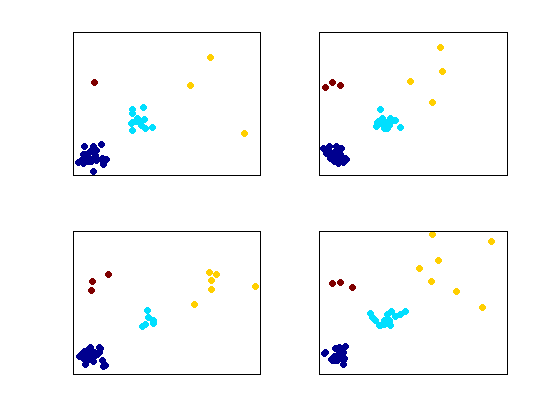
\includegraphics[trim = 4cm 8cm 4cm 8cm, clip, width=5cm]{fig/shared_clustering.pdf}
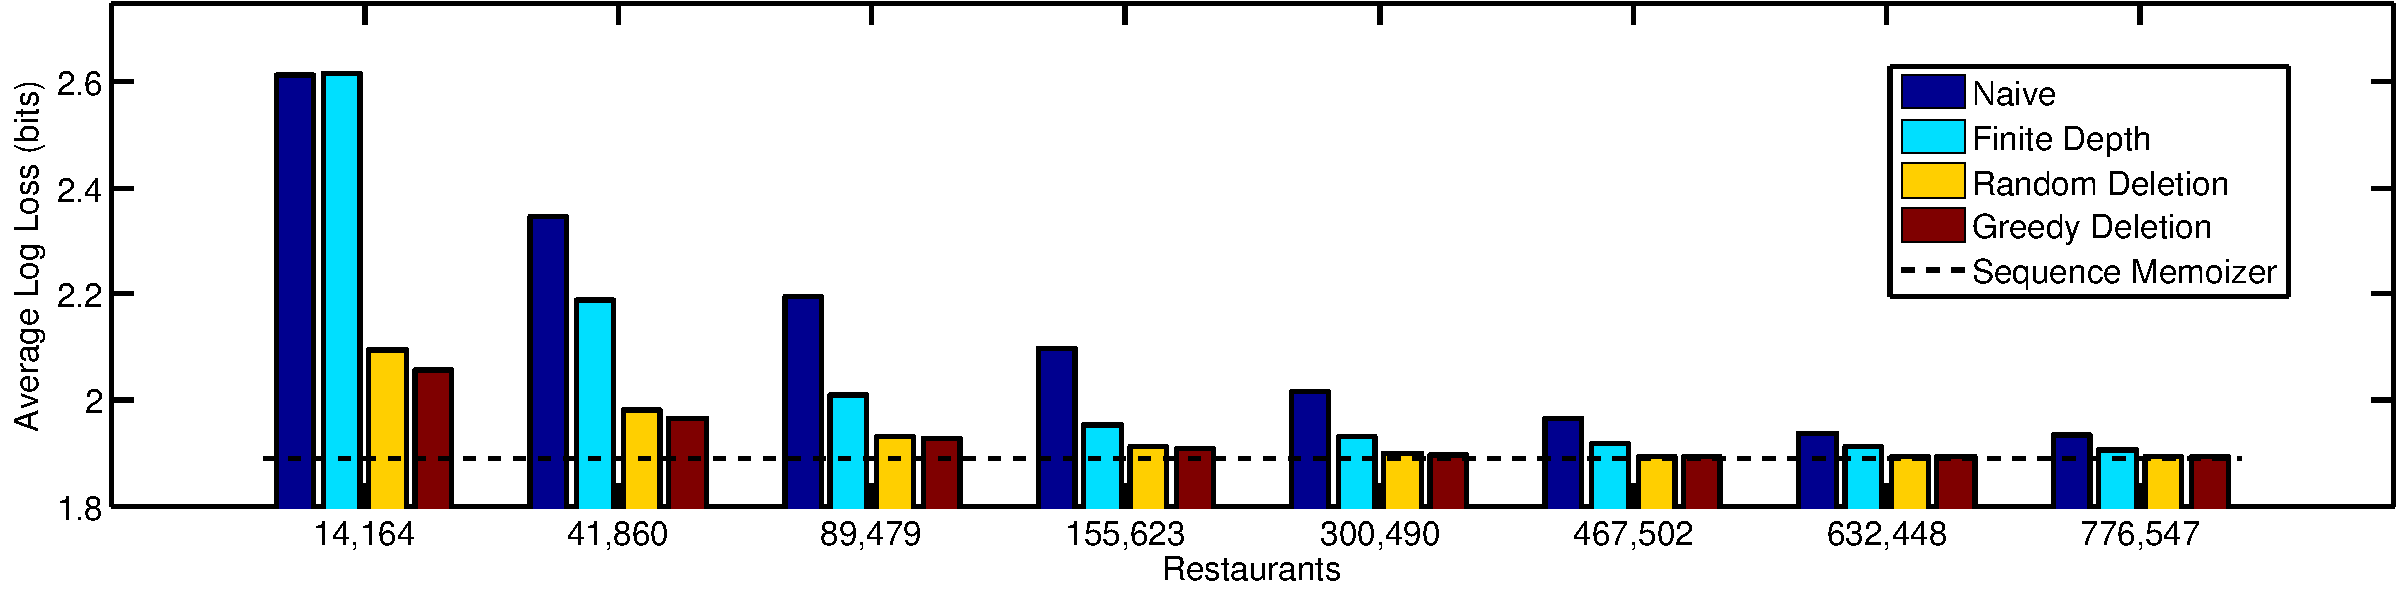
\includegraphics[width=10cm]{../../papers/2010_icml/bounded_memory_compression/results_calgary_corpus.pdf}
%\caption{Shared clustering}
\label{default}
\end{center}
\end{figure}
\begin{itemize}
\item Calgary corpus
\item Different forgetting schemes
\item $256$ character alphabet
\end{itemize}

}
\section{Discussion}
\subsection{Inspiration}
%\frame[t] {%slide 2
 %\frametitle{Inspiration}
%Details, details

%We have a way to regularize joint distributions over sequences of observations
%Method involves hierarchically tying related conditional distributions
%Different factorizations of the joint should be possible.
%Other directions.
 %}

\frame[t] {%slide 2
 \frametitle{Shannon, again$\ldots$}
 ``Prediction and entropy of printed English,'' \citep{Shannon1951}
\begin{quote}
If $[\ldots]$ language is translated into binary digits $[\ldots]$, the entropy H $[\mbox{of the language}]$ is the average number of binary digits required per letter
\end{quote} 
{\begin{center} drppng lttrs dsnt hrt \end{center} }
\begin{quote} $[\ldots]$it appears that, in ordinary literary English, $[\ldots]$ long range statistical effects (up to 100 letters) reduce the entropy to something of the order of one bit per letter
\end{quote}
{\begin{center} d \_ \end{center} }
{\begin{center} the united \_ \end{center} }
{\begin{center} baseball is the national pastime of the united \_ \end{center} }

 }
 \frame[t] {%slide 3
 \frametitle{Inspiration and Reminder}
 Conclusion: lower and upper bound on character-based entropy of English of
$[0.6 < H(English) < 1.3]$ bits per character\footnote{based on a 27 character alphabet, where $log_2(27) \approx 4.75$}\citep{Shannon1951}
 \bigskip
 
 Reminder: 
 \begin{figure}[t]
\begin{center}
%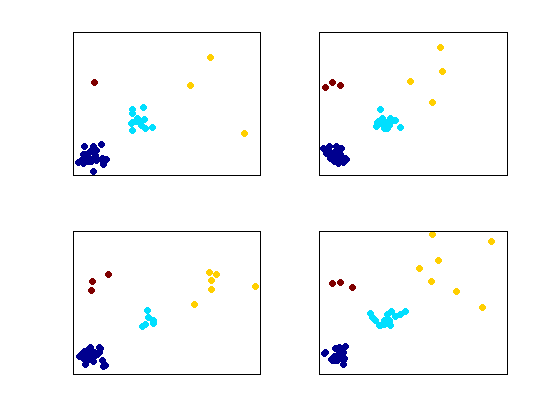
\includegraphics[trim = 4cm 8cm 4cm 8cm, clip, width=5cm]{fig/shared_clustering.pdf}
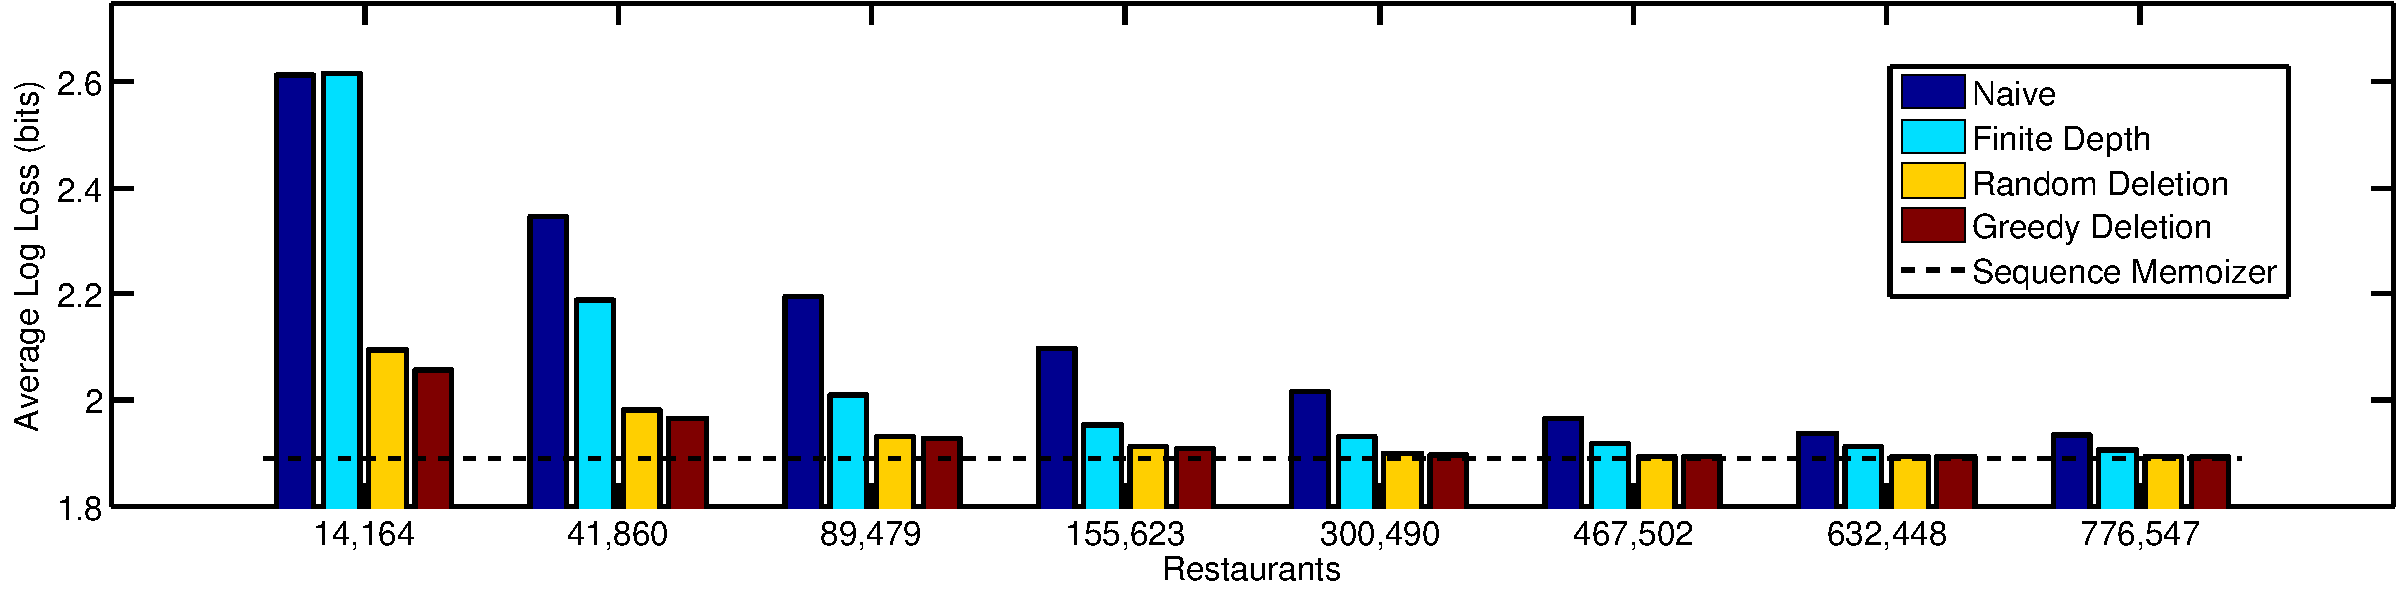
\includegraphics[width=10cm]{../../papers/2010_icml/bounded_memory_compression/results_calgary_corpus.pdf}
%\caption{Shared clustering}
\label{default}
\end{center}
\end{figure}

 
 
\comment{ If $\Sigma$ is a set (an alphabet) and $G$ is a discrete probability distribution over $\Sigma$, (i.e. $\sum_{x\in\Sigma} G(X=x) = 1, 0 < G(x) < 1)$ then you can write the entropy of $G$ as
 
 \[H(G) = -\sum_{x\in\Sigma} G(x) \log_2(G(x))\]
 
 Reminder: entropy is the number of bits per symbol an optimal encoder of a sequence of iid symbols drawn from $G$ would require to losslessly represent the sequence on average. 
 }
 }
 \frame[t] {%slide 4
 \frametitle{Crazy Idea}
 \begin{center}Compression $\approx$ intelligence\end{center}
 ``Text Compression as a Test for Artificial Intelligence,''\cite{Mahoney2009} \newline
 
\begin{quote}The Turing test for artificial intelligence is widely accepted, but is subjective, qualitative, non-repeatable, and difficult to implement. An alternative test without these drawbacks is to insert a machine's language model into a predictive encoder and compress a corpus of natural language text. A ratio of 1.3 bits per character or less indicates that the machine has AI.\end{quote}
 }

 \frame {%slide 4
 \frametitle{Sampling From a Byte Model Trained On NY Times Corpus (3m)}
 bottler , the u.s. college , enjoy a joined his what most again street from all theme oddly produce helped magnet , " " specials , including a pollectioner ) , 7-2ndtake-hns )
the three decades it just happens days to receive branchery , a shadow , " we 've even delight lead to share incoln candidate for the first thing , adaptychicago , " mean tip . phin places like lives in diligenerations , send in the 10 days the airport maytages were on have just happened in 1988 that new york 's spray immediately camps , which print care deal terms , cezanne-manime with largely student can do it is an ec
 }
 
 \frame {%slide 4
 \frametitle{Continuing From a Byte Model Trained On NY Times Corpus (50m)}
{\em the fastest way to make money is$\ldots$}
 being player . bucketti wish i made it end in the reducers and assemblance smart practices to allow city is something to walk in most of the work of agriculture . i 'd be able to compete with an earlier goals : words the danger of conduct in southern california , has set of juice of the fights lack of audience that the eclasm beverly hills . "
she companies or running back down that the book , " grass .
and the coynes , exaggerate between 1972 .
the pad , a debate on emissions on air political capital crashing that the new obviously program " -- irock price , " coach began refugees , much and\footnote{Log-loss 1.49 bits/byte.  2 million rest.'s, forgetting}
 }
  \frame {%slide 4
 \frametitle{Full Circle}
``A Step Towards Fully Unsupervised, Life-Long, Incremental Learning''?
\bigskip

Demonstrated practically useful approach that exhibits
\begin{itemize}
\item Constant space representation $\checkmark$
\item Linear time estimation $\checkmark$
\item Constant time inference $\checkmark$
\end{itemize}
Ways forward?
\begin{itemize}
\item Dependent streams
\item Multi-scale models 
\item Back-off structure learning 
\end{itemize}
 }
\section{Thanks}
 \frame[t] {%slide 5
 \frametitle{Collaborators}
 \begin{itemize}
\item Tom Griffiths
\item Yee Whye Teh
\item Jan Gasthaus
\item Nicholas Bartlett
\item David Pfau
\item Sharon Goldwater
 \end{itemize}
 }	
	%\section{References}	

	\bibliographystyle{plainnat}
	\begin{frame}[t,allowframebreaks]{Bibliograpy}

\bibliography{../../papers/uber}
\end{frame}

\begin{frame}
Special thanks to Ana Calabrese
\end{frame}
\end{document}
